%<<echo=FALSE>>=
%OLD <- options(width=90)
%@
%<<echo=FALSE>>=
%options(OLD) 
%@

\documentclass{beamer}\usepackage[]{graphicx}\usepackage[]{color}
%% maxwidth is the original width if it is less than linewidth
%% otherwise use linewidth (to make sure the graphics do not exceed the margin)
\makeatletter
\def\maxwidth{ %
  \ifdim\Gin@nat@width>\linewidth
    \linewidth
  \else
    \Gin@nat@width
  \fi
}
\makeatother

\definecolor{fgcolor}{rgb}{0.102, 0.102, 0.102}
\newcommand{\hlnum}[1]{\textcolor[rgb]{0.2,0.2,0.2}{#1}}%
\newcommand{\hlstr}[1]{\textcolor[rgb]{0.2,0.2,0.2}{#1}}%
\newcommand{\hlcom}[1]{\textcolor[rgb]{0.302,0.302,0.302}{\textit{#1}}}%
\newcommand{\hlopt}[1]{\textcolor[rgb]{0.102,0.102,0.102}{#1}}%
\newcommand{\hlstd}[1]{\textcolor[rgb]{0.102,0.102,0.102}{#1}}%
\newcommand{\hlkwa}[1]{\textcolor[rgb]{0.102,0.102,0.102}{#1}}%
\newcommand{\hlkwb}[1]{\textcolor[rgb]{0.102,0.102,0.102}{#1}}%
\newcommand{\hlkwc}[1]{\textcolor[rgb]{0.2,0.2,0.2}{#1}}%
\newcommand{\hlkwd}[1]{\textcolor[rgb]{0.102,0.102,0.102}{\textbf{#1}}}%

\usepackage{framed}
\makeatletter
\newenvironment{kframe}{%
 \def\at@end@of@kframe{}%
 \ifinner\ifhmode%
  \def\at@end@of@kframe{\end{minipage}}%
  \begin{minipage}{\columnwidth}%
 \fi\fi%
 \def\FrameCommand##1{\hskip\@totalleftmargin \hskip-\fboxsep
 \colorbox{shadecolor}{##1}\hskip-\fboxsep
     % There is no \\@totalrightmargin, so:
     \hskip-\linewidth \hskip-\@totalleftmargin \hskip\columnwidth}%
 \MakeFramed {\advance\hsize-\width
   \@totalleftmargin\z@ \linewidth\hsize
   \@setminipage}}%
 {\par\unskip\endMakeFramed%
 \at@end@of@kframe}
\makeatother

\definecolor{shadecolor}{rgb}{.97, .97, .97}
\definecolor{messagecolor}{rgb}{0, 0, 0}
\definecolor{warningcolor}{rgb}{1, 0, 1}
\definecolor{errorcolor}{rgb}{1, 0, 0}
\newenvironment{knitrout}{}{} % an empty environment to be redefined in TeX

\usepackage{alltt}% regular slides (with pauses)
%\documentclass[handout]{beamer}% handout (no pauses)

%%%%%%%%%%%%%%%%%%%%%%%%%%%%%%%%%%%%%%%%%%%%%%%%%%%%%%%%%%%%%%%%%%%%%%%%%
%%%%%%% Change the lecture information here %%%%%%%%%%%%%%%%
\def\chapnum{Week \#1}
\title{STAT234: Lecture 1 - Basics of Data Analysis !!}
\author{Kushal K. Dey}
\date{}
%%%%%%%%%%%%%%%%%%%%%%%%%%%%%%%%%%%%%%%%%%%%%%%%%%%%%%%%%%%%%%%%%%%%%%%%%

%%%%%% Start of suggested definitions and packages %%%%%%%%%%%%
%%%%%% Do not change unless you really know what you are doing %%%%%%%%%%
%%%%%%%%%%%%%%%%%%%%%%%%%%%%%%%%%%%%%%%%%%%%%%%%%%%%%%%%%%%%%%%%%%%%%%%%%

\usepackage{enumerate}
\usepackage{amsmath, bbm}
\usepackage[misc]{ifsym} % for the dice symbol \Cube{}
\usepackage[latin1]{inputenc}
\usepackage{hyperref}

%\usepackage{comment}
%\usepackage{pstricks}
%\usepackage{graphicx}
%\usepackage{booktabs}
%\usepackage{pgfpages}
%\pgfpagesuselayout{2 on 1}[a4paper,border shrink=3mm]
%\pgfpagesuselayout{4 on 1}[a4paper,landscape,border shrink=3mm

\usepackage{setspace}
\ifdefined\knitrout
  \renewenvironment{knitrout}{\begin{spacing}{0.75}\begin{tiny}}{\end{tiny}\end{spacing}}
\else
\fi

%%%%%%%%%%%%%%% Defined Shortcuts (macros) %%%%%%%%%%%%%
% parameters and statistics
\newcommand{\xbar}{\overline{x}}
\newcommand{\Xbar}{\overline{X}}
\newcommand{\ybar}{\overline{y}}
\newcommand{\Ybar}{\overline{Y}}
\newcommand{\dbar}{\overline{d}}
\newcommand{\Dbar}{\overline{D}}
\newcommand{\zbar}{\overline{z}}
\newcommand{\Zbar}{\overline{Z}}
\newcommand{\ehat}{\widehat{\epsilon}}
\newcommand{\yhat}{\widehat{y}}
\newcommand{\Yhat}{\widehat{Y}}
\newcommand{\betaa}{{\beta_0}}
\newcommand{\betab}{{\beta_1}}
\newcommand{\betac}{{\beta_2}}
\newcommand{\betad}{{\beta_3}}
\newcommand{\BETA}{{\boldsymbol\beta}}
\newcommand{\betahata}{\widehat{\beta_0}}
\newcommand{\betahatb}{\widehat{\beta_1}}
\newcommand{\betahatc}{\widehat{\beta_2}}
\newcommand{\betahatd}{\widehat{\beta_3}}
\newcommand{\bhat}{\widehat{b}}
\newcommand{\btilde}{\widetilde{b}}
\newcommand{\ahat}{\widehat{a}}
\newcommand{\atilde}{\widetilde{a}}
\newcommand{\rss}{\mathit{SSE}}
\newcommand{\sigmahat}{\widehat{\sigma}}
\newcommand{\betahat}{\widehat{\beta}}
\newcommand{\thetahat}{\widehat{\theta}}
\newcommand{\phat}{\widehat{p}}
\newcommand{\pihat}{\widehat{\pi}}
\newcommand{\muhat}{\widehat{\mu}}
% real numbers and integers
\newcommand{\reals}{\mathbbm{R}}
\newcommand{\integers}{\mathbbm{N}}
%distributions
\newcommand{\normal}{\textsf{Norm}}
\newcommand{\Bin}{\textsf{Binom}}
\newcommand{\Uni}{\textsf{Unif}}
\newcommand{\Poisson}{\textsf{Pois}}
\newcommand{\Exp}{\textsf{Exp}}
\newcommand{\Beta}{\textsf{Beta}}
\newcommand{\iid}{\stackrel{\mathrm{iid}}{\sim}}
% probability and expected value
\newcommand{\rv}{r.v.\ }
\newcommand{\prob}{{\rm P}}
\newcommand{\mean}{\mathrm{E}}
\newcommand{\var}{\mathrm{Var}}
\newcommand{\Var}{\mathrm{Var}}
\newcommand{\cov}{\mathrm{Cov}}
\newcommand{\corr}{\mathop{\mathrm{Corr}}}
% measures of spread
\newcommand{\IQR}{\textit{IQR}}
\newcommand{\SAD}{\textit{SAD}}
\newcommand{\MAD}{\textit{MAD}}
\newcommand{\SSD}{\textit{SSD}}
\newcommand{\MSD}{\textit{MSD}}
\newcommand{\RMSD}{\textit{RMSD}}
\newcommand{\MSE}{\textit{MSE}}
\newcommand{\MSR}{\textit{MSR}}
% formatting code and such
\providecommand{\variable}[1]{}
\renewcommand{\variable}[1]{{\color{green!50!black}\texttt{#1}}}
\providecommand{\function}[1]{}
\renewcommand{\function}[1]{{\color{purple!75!blue}\texttt{\StrSubstitute{#1}{()}{}()}}}
\providecommand{\option}[1]{}
\renewcommand{\option}[1]{{\color{brown!80!black}\texttt{#1}}}
\providecommand{\pkg}[1]{}
\renewcommand{\pkg}[1]{{\color{red!80!black}\texttt{#1}}}
\providecommand{\code}[1]{}
\renewcommand{\code}[1]{{\color{blue!80!black}\texttt{#1}}}

%%%%%%%%%
% Changed by Kushal K Dey, University of Chicago
%\providecommand{\file}[1]{}
%\renewcommand{\file}[1]{{\tt #1}}
\providecommand{\file}[1]{}
\renewcommand{\file}[1]{{\color{orange!80!black}\texttt{#1}}}
%\providecommand{\dataframe}[1]{}
%\renewcommand{\dataframe}[1]{{\color{blue!80!black}\texttt{#1}}}
\providecommand{\dataframe}[1]{}
\renewcommand{\dataframe}[1]{{\color{cyan!80!black}\texttt{#1}}}
%%%%%%%%%

% other
\def\Sum{\sum\nolimits}
\def\b#1{\fboxsep=0pt\colorbox{black}{\color{white}\Cube{#1}}}
\def\w#1{\Cube{#1}}
%%%%%%%%%%%% End of shortcuts (macros) ##############

%%%%%%%%% One way to hide answers until you want to show them %%%%%%%%%
\def\Hide#1#2{\ul{~~~\onslide<#1>{\alert{#2}}~~~}}
\def\hide#1#2{\ul{~~\onslide<#1>{\alert{#2}}~~}}
\def\hid#1#2{\onslide<#1>{\alert{#2}}}
% Choose the color of answers here too
\setbeamercolor{alerted text}{fg=darkgray} 
%\setbeamercolor{alerted text}{fg=black} 

%------Centered Page Number Setup ------
\defbeamertemplate{footline}{centered page number}
{%
  \hspace*{\fill}%
  %\usebeamercolor[fg]{page number in head/foot}%
  %\usebeamerfont{page number in head/foot}%
  \tiny \chapnum: Page \insertframenumber\, of \inserttotalframenumber%
  \hspace*{\fill}\vskip2pt%
}
%\setbeamertemplate{footline}{\hfill\insertframenumber/\inserttotalframenumber}
\setbeamertemplate{footline}[centered page number]
%--------------------------------

%\usetheme{Copenhagen}
\setbeamertemplate{navigation symbols}{}
\usepackage[english]{babel}
\def\ul{\underline}
\linespread{1.1}
% or whatever



%\parskip=0pt
\IfFileExists{upquote.sty}{\usepackage{upquote}}{}
\begin{document}%large

%<<setup, include=FALSE, cache=FALSE>>=
%options(replace.assign=TRUE,width=90, digits=4)
%opts_chunk$set(fig.path='figure/graphics-', cache.path='cache/graphics-', fig.align='center', fig.width=8, fig.height=5.5, fig.show='as.is', out.width='0.9\\linewidth', cache=FALSE, par=TRUE, size = 'tiny', tidy=TRUE, cache.extra=rand_seed)
%knit_hooks$set(par=function(before, options, envir){
%if (before && options$fig.show!='none') par(mar=c(4,4,.1,.1),cex.lab=.95,cex.axis=.9,mgp=c(2,.7,0),tcl=-.3)
%}, document = function(x) {
%  gsub('\\\\(begin|end)\\{kframe\\}', '', x)
%}, crop=hook_pdfcrop)
%@
%<<setup2, include=FALSE, cache=FALSE>>=
%knit_theme$set("print")
%@


%%%%%%%%%%%%%%%%%%%%%%%%%%%%%%%%%%%%%%%%%%%%%%%%%%%%%%%%%%%%%%%%%%%%%%%%%
%%%%%%%%%%%%%%%%%%%%%%%%%%%%%%%%%%%%%%%%%%%%%%%%%%%%%%%%%%%%%%%%%%%%%%%%%
%%%%%% End of suggested definitions and packages %%%%%%%%%%%%

%------------------------------------------------------------------
%------------------------------------------------------------------

%%%%%%%%%% Title frame (optional) %%%%%%%%%%%%%
\begin{frame}{}
\maketitle
\end{frame}
%%%%%%%%%%%%%%%%%%%%%%%%%%%%%%%%%%%%%%%%%%%%%%%

%%%%%%%%%%%%%% Begin slides here %%%%%%%%%%%%%%
\begin{frame}[fragile]
%%%%%%%%%%%%%%%%%%%%%%%%%%%%%%%%%%%%%%%%%%%%%%%
\frametitle{Requisites}

Main software for this course: R and RStudio \pause \newline

Rstudio Installation: 
\url{http://statistics.uchicago.edu/~collins/Rinstall/} \pause \newline 

You would need to load the package \emph{mosaic} every time
you start R. \pause \newline

Office hour time (7 sessions) + Problem session (4 hrs) each week:
Timings to be decided later
\end{frame}

%%%%%%%%%%%%%%%%%%%%%%%%%%%%%%%%%%%%%%%%%%%%%%%%%%%%%%%%%%%%
\begin{frame}[fragile]
%%%%%%%%%%%%%%%%%%%%%%%%%%%%%%%%%%%%%%%%%%%%%%%%%%%%%%%%%%%%
\frametitle{Let's Start!}

What is Data? \pause\newline
Simply put, a collection of facts that can be analyzed !  
\newline \pause

Collection and analysis of data is called \textit{statistics}. \pause \newline

Where can I get data?\pause\newline
Everywhere! ....well almost!
\newline\pause 
 

Examples:  \pause (Rather questions ! )
\pause
\begin{itemize}
\item How many apps do you have on your phone? \pause
\item How much money did you spend on lunch? \pause 
\item How What grade did you get in STAT 234? \pause
\end{itemize}

\end{frame}
%%%%%%%%%%%%%%%%%%%%%%%%%%%%%%%%%%%%%%%%%%%%%%%%%%%%%%%%%%%%

%%%%%%%%%%%%%%%%%%%%%%%%%%%%%%%%%%%%%%%%%%%%%%%%%%%%%%%%%%%%
\begin{frame}[fragile]
%%%%%%%%%%%%%%%%%%%%%%%%%%%%%%%%%%%%%%%%%%%%%%%%%%%%%%%%%%%%
\frametitle{Backdrop}

Beginning of Statistics? \pause\newline
1532 $\rightarrow$ First weekly data on deaths in London (Sir W. Petty) \newline
1539 $\rightarrow$ Data collection on marriages, baptism and death in France
1654 $\rightarrow$ Correspondence with gambling and probability (Fermat and Pascal)
\newline \pause

Topics covered in this course will focus on the period between 1890s-1960s.
\newline \pause 

Recently there is a lot of interest in Data Science and Big Data Analysis, which
are essentially applying statistics on data of large size (many GBs or TBs). For example, Facebook, Twitter and Google generates massive data of user activity 
for billions of users daily!

\end{frame}

%%%%%%%%%%%%%%%%%%%%%%%%%%%%%%%%%%%%%%%%%%%%%%%%%%%%%%%%%%%%
\begin{frame}[fragile]
%%%%%%%%%%%%%%%%%%%%%%%%%%%%%%%%%%%%%%%%%%%%%%%%%%%%%%%%%%%%
\frametitle{Lets look at some Data!!}

As a toy exercise, lets analyze twitter feed of..... \pause \newline

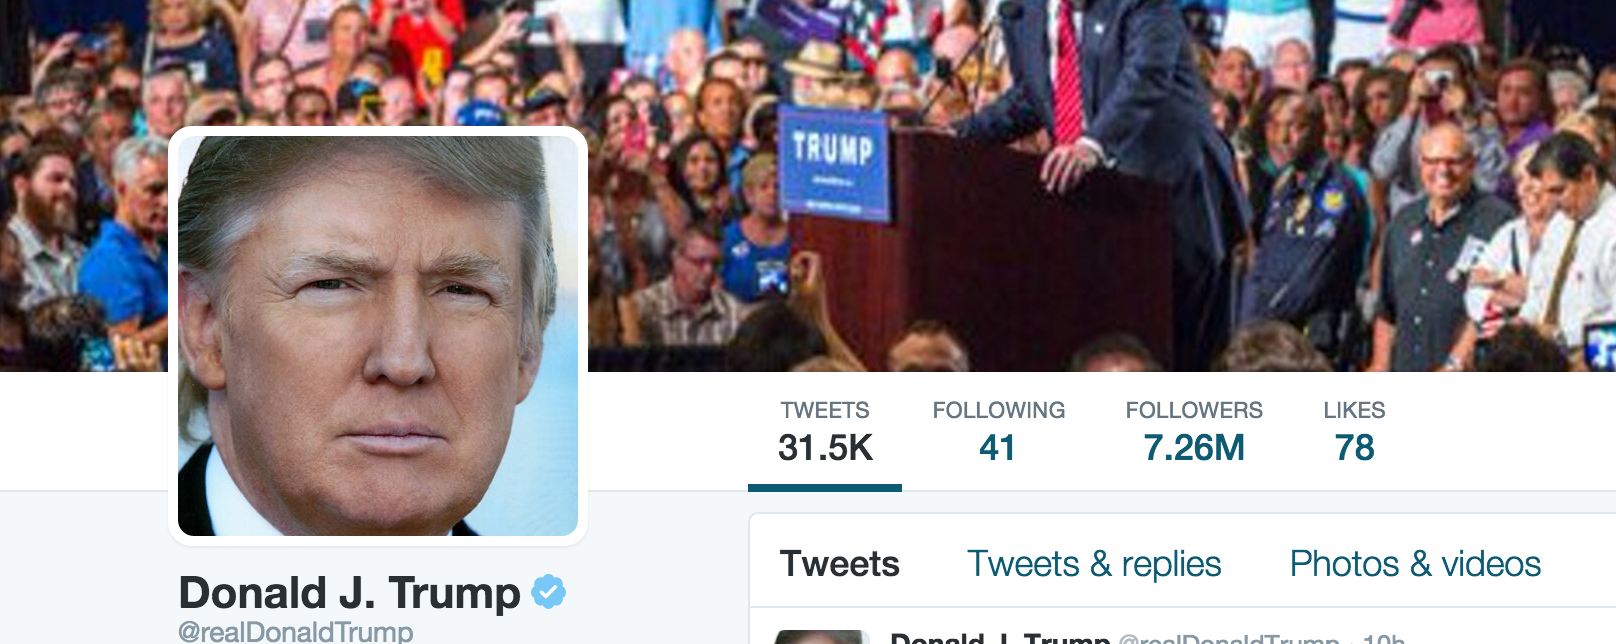
\includegraphics[width=8cm,keepaspectratio]{trump.png}

Load the data 





\begin{knitrout}\small
\definecolor{shadecolor}{rgb}{1, 1, 1}\color{fgcolor}\begin{kframe}
\begin{alltt}
\hlcom{#library(devtools); install_github('kkdey/TrumpTwitterFeed')}
\hlkwd{library}\hlstd{(TrumpTwitterFeed)}
\hlkwd{data}\hlstd{(}\hlstr{"trump.data.frame"}\hlstd{)}
\hlkwd{dim}\hlstd{(trump.data.frame)}
\end{alltt}
\begin{verbatim}
[1] 1336    6
\end{verbatim}
\end{kframe}
\end{knitrout}
\end{frame}

%%%%%%%%%%%%%%%%%%%%%%%%%%%%%%%%%%%%%%%%%%%%%%%%%%%%%%%%%%%%
\begin{frame}[fragile]
%%%%%%%%%%%%%%%%%%%%%%%%%%%%%%%%%%%%%%%%%%%%%%%%%%%%%%%%%%%%
\frametitle{Snapshot of the Data-1}

\begin{knitrout}\small
\definecolor{shadecolor}{rgb}{1, 1, 1}\color{fgcolor}\begin{kframe}
\begin{alltt}
\hlkwd{head}\hlstd{(trump.data.frame[,}\hlnum{1}\hlopt{:}\hlnum{5}\hlstd{],} \hlnum{3}\hlstd{)}
\end{alltt}
\begin{verbatim}
  tweet_month tweet_year tweet_day retweets favorites
1    2016-Mar       2016        26     7625     24147
2    2016-Mar       2016        26     6412     19867
3    2016-Mar       2016        26     4773     15029
\end{verbatim}
\begin{alltt}
\hlkwd{tail}\hlstd{(trump.data.frame[,}\hlnum{1}\hlopt{:}\hlnum{5}\hlstd{],} \hlnum{3}\hlstd{)}
\end{alltt}
\begin{verbatim}
     tweet_month tweet_year tweet_day retweets favorites
1334    2015-Oct       2015        13      732      1640
1335    2015-Oct       2015        13      974      2254
1336    2015-Oct       2015        13     4578      8393
\end{verbatim}
\end{kframe}
\end{knitrout}

\end{frame}

%%%%%%%%%%%%%%%%%%%%%%%%%%%%%%%%%%%%%%%%%%%%%%%%%%%%%%%%%%%%
\begin{frame}[fragile]
%%%%%%%%%%%%%%%%%%%%%%%%%%%%%%%%%%%%%%%%%%%%%%%%%%%%%%%%%%%%
\frametitle{Snapshot of the Data- 2}

\begin{knitrout}\small
\definecolor{shadecolor}{rgb}{1, 1, 1}\color{fgcolor}\begin{kframe}
\begin{alltt}
\hlkwd{glimpse}\hlstd{(trump.data.frame)}
\end{alltt}
\begin{verbatim}
Observations: 1,336
Variables: 6
$ tweet_month (fctr) 2016-Mar, 2016-Mar, 2016-Mar, 2016...
$ tweet_year  (fctr) 2016, 2016, 2016, 2016, 2016, 2016...
$ tweet_day   (fctr) 26, 26, 26, 26, 26, 26, 26, 26, 26...
$ retweets    (dbl) 7625, 6412, 4773, 7079, 5143, 5374,...
$ favorites   (dbl) 24147, 19867, 15029, 20798, 15922, ...
$ tweet_text  (fctr) Remember, I am the only candidate ...
\end{verbatim}
\begin{alltt}
\hlkwd{summary}\hlstd{(trump.data.frame)}
\end{alltt}
\begin{verbatim}
   tweet_month  tweet_year   tweet_day      retweets    
 2015-Oct: 93   2015:434   03     : 93   Min.   :  322  
 2015-Nov:138   2016:902   28     : 89   1st Qu.: 1270  
 2015-Dec:203              12     : 75   Median : 2356  
 2016-Jan:226              24     : 70   Mean   : 3113  
 2016-Feb:324              23     : 69   3rd Qu.: 4130  
 2016-Mar:352              15     : 68   Max.   :25524  
                           (Other):872                  
   favorites    
 Min.   :  713  
 1st Qu.: 3729  
 Median : 6905  
 Mean   : 8647  
 3rd Qu.:11610  
 Max.   :47724  
                
                                                                                                                                      tweet_text  
 MAKE AMERICA GREAT AGAIN!                                                                                                                 :   7  
 . #JoeTheismann was great as a political analyst on @FoxNews. He knows far more than football. Thanks for the nice words Joe!             :   1  
 .@andersoncooper did an excellent job of hosting the #DemDebate last night. Tough, firm, but fair.                                        :   1  
 .@AndreaTantaros- You are a true journalistic professional. I so agree with what you say. Keep up the great work! #MakeAmericaGreatAgain  :   1  
 .@AnnCoulter has been amazing. We will win and establish strong borders, we will build a WALL and Mexico will pay. We will be great again!:   1  
 .@AP is doing very badly. I can say from experience their reporting is terrible &amp; highly inaccurate. Sadly, they are now irrelevant!  :   1  
 (Other)                                                                                                                                   :1324  
\end{verbatim}
\end{kframe}
\end{knitrout}

\end{frame}

%%%%%%%%%%%%%%%%%%%%%%%%%%%%%%%%%%%%%%%%%%%%%%%%%%%%%%%%%%%%
\begin{frame}[fragile]
%%%%%%%%%%%%%%%%%%%%%%%%%%%%%%%%%%%%%%%%%%%%%%%%%%%%%%%%%%%%
\frametitle{Sorting number of retweets}

\begin{knitrout}\small
\definecolor{shadecolor}{rgb}{1, 1, 1}\color{fgcolor}\begin{kframe}
\begin{alltt}
\hlstd{sorted_retweet_counts} \hlkwb{<-} \hlkwd{sort}\hlstd{(trump.data.frame}\hlopt{$}\hlstd{retweets)}


\hlkwd{tail}\hlstd{(sorted_retweet_counts)}
\end{alltt}
\begin{verbatim}
[1] 18287 18303 18638 19252 25323 25524
\end{verbatim}
\begin{alltt}
\hlkwd{head}\hlstd{(sorted_retweet_counts)}
\end{alltt}
\begin{verbatim}
[1] 322 375 412 418 439 455
\end{verbatim}
\end{kframe}
\end{knitrout}

\end{frame}

%%%%%%%%%%%%%%%%%%%%%%%%%%%%%%%%%%%%%%%%%%%%%%%%%%%%%%%%%%%%
\begin{frame}[fragile]
%%%%%%%%%%%%%%%%%%%%%%%%%%%%%%%%%%%%%%%%%%%%%%%%%%%%%%%%%%%%
\frametitle{Sorting number of retweets}

\begin{knitrout}\small
\definecolor{shadecolor}{rgb}{1, 1, 1}\color{fgcolor}\begin{kframe}
\begin{alltt}
\hlkwd{quantile}\hlstd{(}\hlopt{~}\hlstd{retweets,} \hlkwc{data}\hlstd{=trump.data.frame)}
\end{alltt}
\begin{verbatim}
   0%   25%   50%   75%  100% 
  322  1270  2356  4130 25524 
\end{verbatim}
\end{kframe}
\end{knitrout}

IQR or inter-quartile range is the difference between the $75$ th quantile and the 
$25$ tquantile.

\begin{knitrout}\small
\definecolor{shadecolor}{rgb}{1, 1, 1}\color{fgcolor}\begin{kframe}
\begin{alltt}
\hlkwd{IQR}\hlstd{(}\hlopt{~}\hlstd{retweets,} \hlkwc{data}\hlstd{=trump.data.frame)}
\end{alltt}
\begin{verbatim}
[1] 2860
\end{verbatim}
\end{kframe}
\end{knitrout}

\end{frame}

%%%%%%%%%%%%%%%%%%%%%%%%%%%%%%%%%%%%%%%%%%%%%%%%%%%%%%%%%%%%
\begin{frame}[fragile]
%%%%%%%%%%%%%%%%%%%%%%%%%%%%%%%%%%%%%%%%%%%%%%%%%%%%%%%%%%%%
\frametitle{Box plot of retweets}

\begin{knitrout}\small
\definecolor{shadecolor}{rgb}{1, 1, 1}\color{fgcolor}\begin{kframe}
\begin{alltt}
\hlkwd{bwplot}\hlstd{(}\hlopt{~} \hlstd{retweets,} \hlkwc{data}\hlstd{=trump.data.frame,}
       \hlkwc{xlab}\hlstd{=}\hlstr{"Retweets box plot distribution"}\hlstd{)}
\end{alltt}
\end{kframe}

{\centering 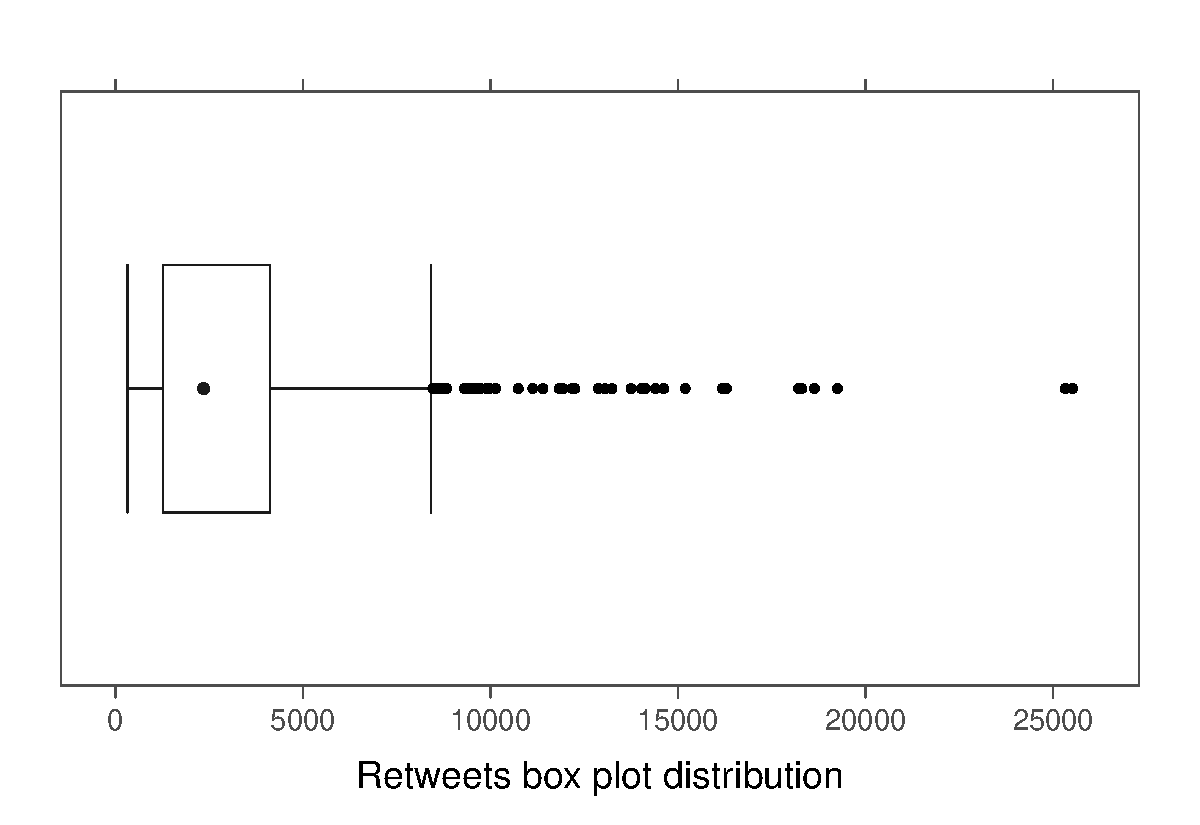
\includegraphics[width=0.99\linewidth]{figure/graphics-bw_retweets-1} 

}



\end{knitrout}

\end{frame}

%%%%%%%%%%%%%%%%%%%%%%%%%%%%%%%%%%%%%%%%%%%%%%%%%%%%%%%%%%%%
\begin{frame}[fragile]
%%%%%%%%%%%%%%%%%%%%%%%%%%%%%%%%%%%%%%%%%%%%%%%%%%%%%%%%%%%%
\frametitle{Bar graph}

\begin{knitrout}\small
\definecolor{shadecolor}{rgb}{1, 1, 1}\color{fgcolor}\begin{kframe}
\begin{alltt}
\hlkwd{bargraph}\hlstd{(retweets} \hlopt{~} \hlstd{tweet_month,} \hlkwc{data}\hlstd{=trump.data.frame,}
   \hlkwc{type}\hlstd{=}\hlstr{"percent"}\hlstd{,} \hlkwc{xlab}\hlstd{=}\hlstr{"Trump Retweets by month"}\hlstd{,} \hlkwc{cex}\hlstd{=}\hlnum{0.5}\hlstd{)}
\end{alltt}
\end{kframe}

{\centering 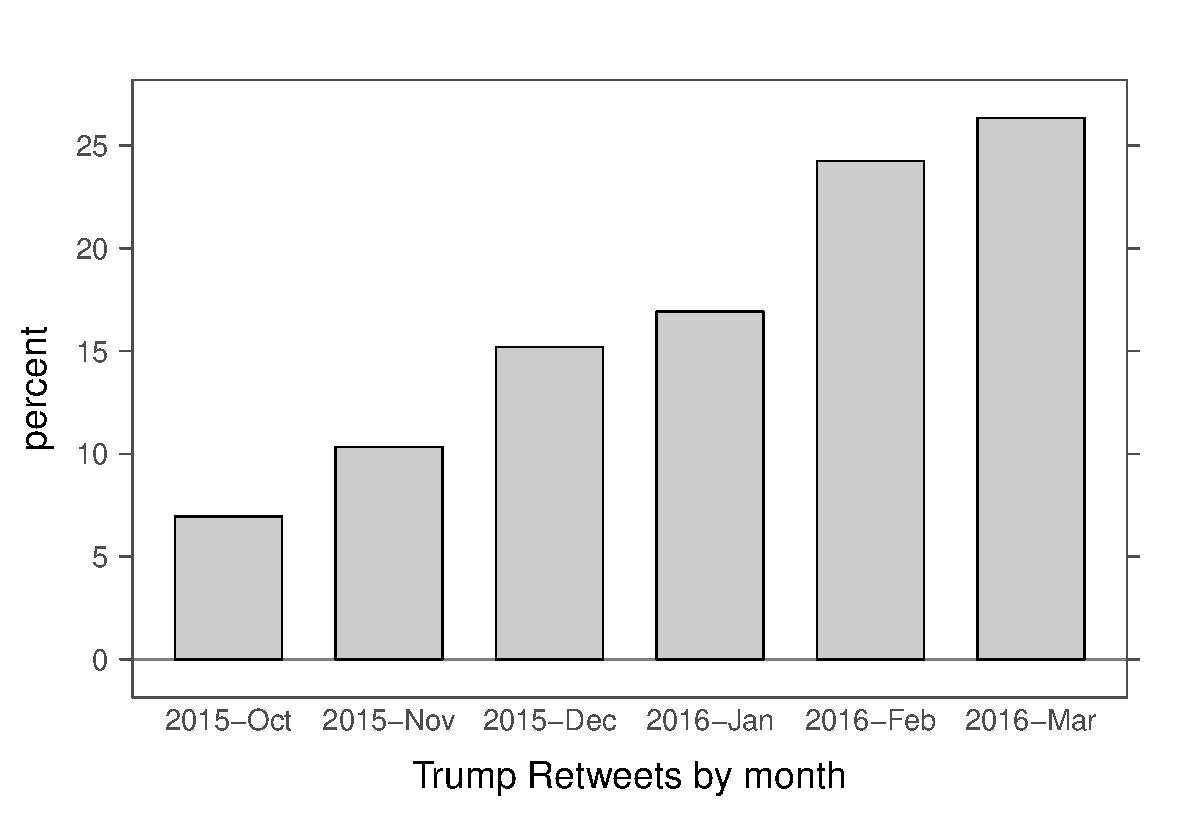
\includegraphics[width=0.99\linewidth]{figure/graphics-bar_retweets_1-1} 

}



\end{knitrout}

\end{frame}

%%%%%%%%%%%%%%%%%%%%%%%%%%%%%%%%%%%%%%%%%%%%%%%%%%%%%%%%%%%%
\begin{frame}[fragile]
%%%%%%%%%%%%%%%%%%%%%%%%%%%%%%%%%%%%%%%%%%%%%%%%%%%%%%%%%%%%
\frametitle{Bar graph}

\begin{knitrout}\small
\definecolor{shadecolor}{rgb}{1, 1, 1}\color{fgcolor}\begin{kframe}
\begin{alltt}
\hlkwd{bargraph}\hlstd{(retweets} \hlopt{~} \hlstd{tweet_year,}
         \hlkwc{data}\hlstd{=trump.data.frame,} \hlkwc{type}\hlstd{=}\hlstr{"percent"}\hlstd{,}
          \hlkwc{xlab}\hlstd{=}\hlstr{"Trump Retweets by years"}\hlstd{,} \hlkwc{cex}\hlstd{=}\hlnum{0.5}\hlstd{)}
\end{alltt}
\end{kframe}

{\centering 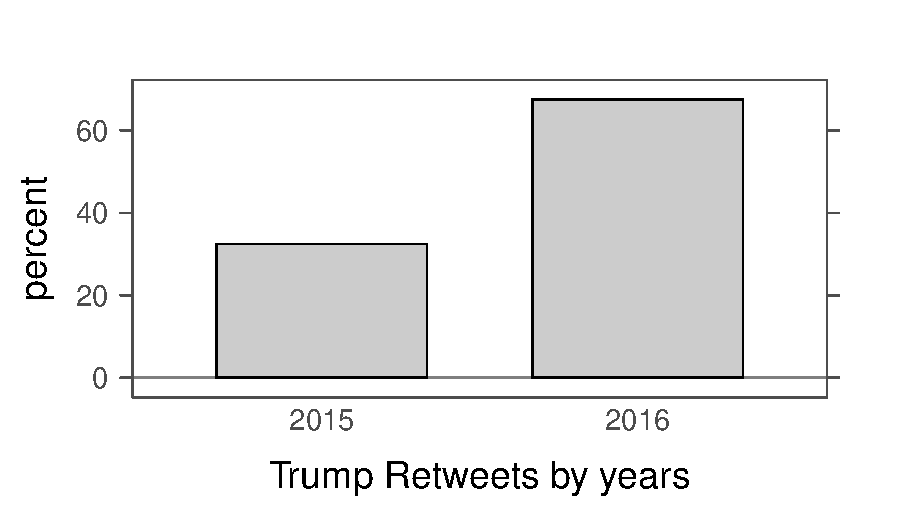
\includegraphics[width=0.99\linewidth]{figure/graphics-bar_retweets_2-1} 

}



\end{knitrout}

\end{frame}

%%%%%%%%%%%%%%%%%%%%%%%%%%%%%%%%%%%%%%%%%%%%%%%%%%%%%%%%%%%%
\begin{frame}[fragile]
%%%%%%%%%%%%%%%%%%%%%%%%%%%%%%%%%%%%%%%%%%%%%%%%%%%%%%%%%%%%
\frametitle{Bar graph}

\begin{knitrout}\small
\definecolor{shadecolor}{rgb}{1, 1, 1}\color{fgcolor}\begin{kframe}
\begin{alltt}
\hlkwd{bargraph}\hlstd{(retweets}\hlopt{~} \hlstd{tweet_day} \hlopt{|} \hlstd{tweet_year,}
         \hlkwc{data}\hlstd{=trump.data.frame,} \hlkwc{type}\hlstd{=}\hlstr{"percent"}\hlstd{,}
         \hlkwc{xlab}\hlstd{=}\hlstr{"Trump Retweets by days in years"}\hlstd{,}
         \hlkwc{ylab}\hlstd{=}\hlstr{"Percent"}\hlstd{,} \hlkwc{layout}\hlstd{=}\hlkwd{c}\hlstd{(}\hlnum{1}\hlstd{,}\hlnum{2}\hlstd{))}
\end{alltt}
\end{kframe}

{\centering 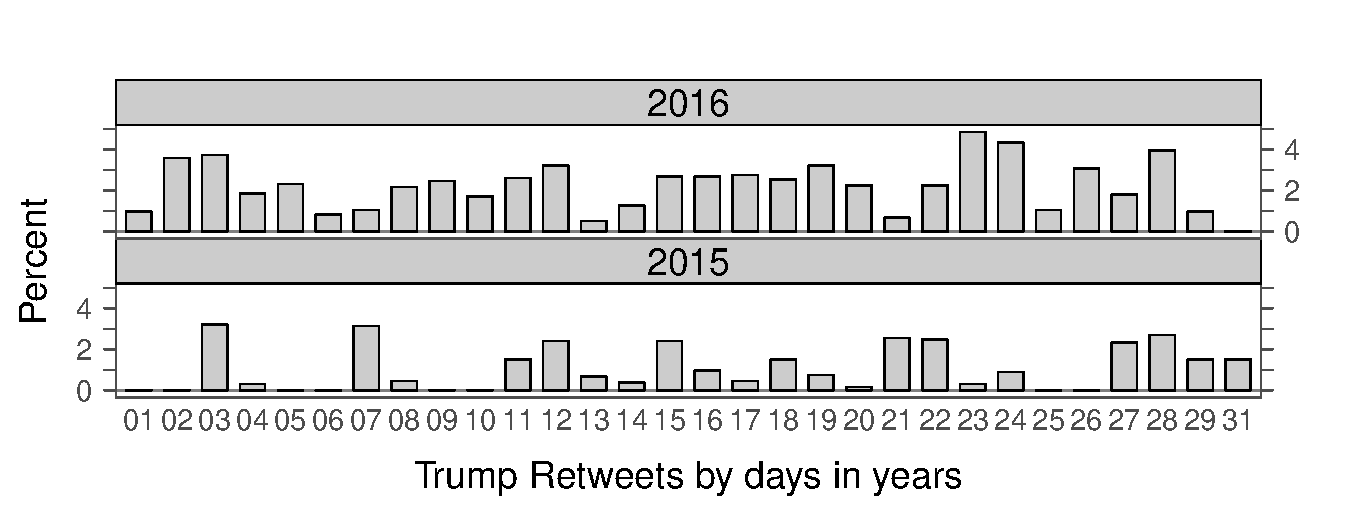
\includegraphics[width=0.99\linewidth]{figure/graphics-bar_retweets_3-1} 

}



\end{knitrout}

\end{frame}

%%%%%%%%%%%%%%%%%%%%%%%%%%%%%%%%%%%%%%%%%%%%%%%%%%%%%%%%%%%%
\begin{frame}[fragile]
%%%%%%%%%%%%%%%%%%%%%%%%%%%%%%%%%%%%%%%%%%%%%%%%%%%%%%%%%%%%
\frametitle{Histogram}

\begin{knitrout}\small
\definecolor{shadecolor}{rgb}{1, 1, 1}\color{fgcolor}\begin{kframe}
\begin{alltt}
\hlkwd{histogram}\hlstd{(retweets} \hlopt{~} \hlstd{tweet_month,} \hlkwc{data}\hlstd{=trump.data.frame,}
          \hlkwc{type}\hlstd{=}\hlstr{"percent"}\hlstd{,} \hlkwc{xlab}\hlstd{=}\hlstr{"Trump Retweets per month"}\hlstd{)}
\end{alltt}
\end{kframe}

{\centering 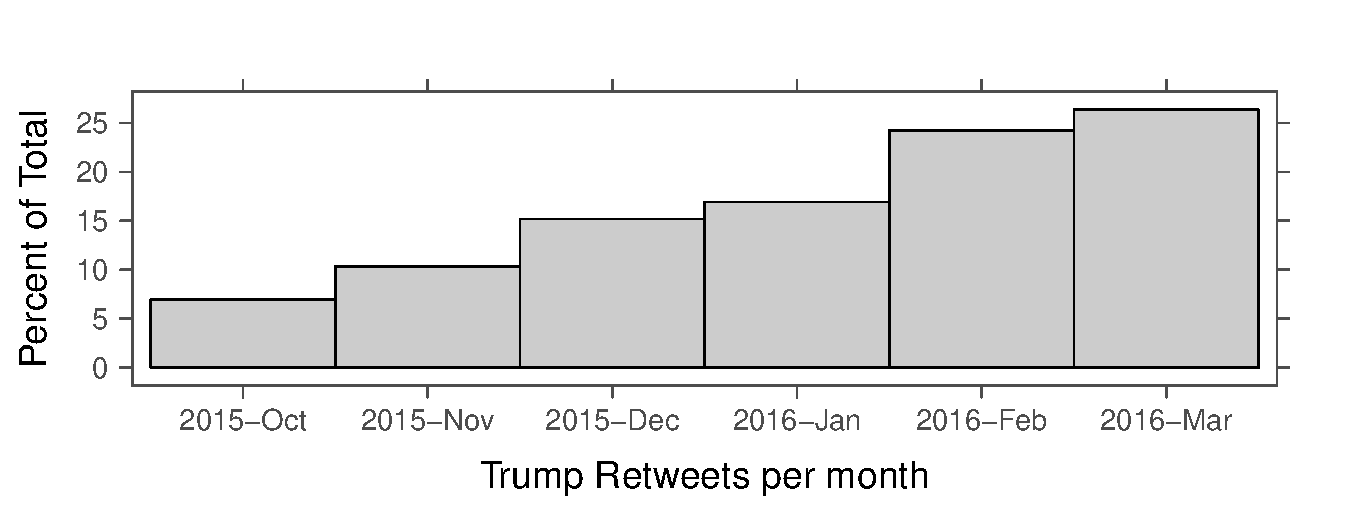
\includegraphics[width=0.99\linewidth]{figure/graphics-histogram-1} 

}



\end{knitrout}

\end{frame}

%%%%%%%%%%%%%%%%%%%%%%%%%%%%%%%%%%%%%%%%%%%%%%%%%%%%%%%%%%%%
\begin{frame}[fragile]
%%%%%%%%%%%%%%%%%%%%%%%%%%%%%%%%%%%%%%%%%%%%%%%%%%%%%%%%%%%%
\frametitle{Scatter Plot}

\begin{knitrout}\small
\definecolor{shadecolor}{rgb}{1, 1, 1}\color{fgcolor}\begin{kframe}
\begin{alltt}
\hlkwd{scatter.smooth}\hlstd{(trump.data.frame}\hlopt{$}\hlstd{retweets,}
      \hlstd{trump.data.frame}\hlopt{$}\hlstd{favorites,} \hlkwc{lwd}\hlstd{=}\hlnum{1}\hlstd{,} \hlkwc{pch}\hlstd{=}\hlnum{20}\hlstd{,}
      \hlkwc{col}\hlstd{=}\hlstr{"blue"}\hlstd{,}\hlkwc{xlab}\hlstd{=}\hlstr{"Retweets"}\hlstd{,} \hlkwc{ylab}\hlstd{=}\hlstr{"Favorites"}\hlstd{)}
\end{alltt}
\end{kframe}

{\centering 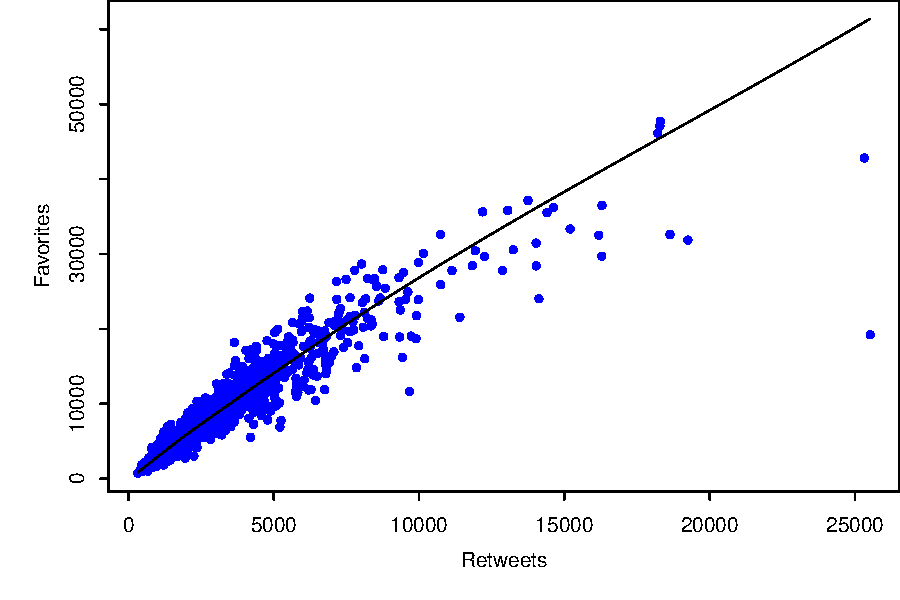
\includegraphics[width=0.99\linewidth]{figure/graphics-scatter-1} 

}



\end{knitrout}

\end{frame}

%%%%%%%%%%%%%%%%%%%%%%%%%%%%%%%%%%%%%%%%%%%%%%%%%%%%%%%%%%%%
\begin{frame}[fragile]{The Average is the Balancing Point\;\;}
%%%%%%%%%%%%%%%%%%%%%%%%%%%%%%%%%%%%%%%%%%%%%%%%%%%%%%%%%%%%
\vspace{0.25cm}

Consider the data $x_1=9, x_2=3, x_3=15, x_4=1$
\begin{itemize}
\item What is the average of these values?
\pause
\item What are the deviations of the data from the average?
\pause
\item What is the sum of the deviations from the average?
\pause
\item The average is the ``balancing point" of the data, the ``center of mass" (assigning each data value the same mass = $1/4$)
\end{itemize}
\vskip0.5cm
\pause
Talk a moment with your neighbor.  See if you can 
come up an equation to express this ``balancing point"
property of the average.
\vskip0.5cm
\pause
\textbf{Proof:} Show that for \textbf{any} sample of size $n,$
\;\;$\displaystyle{\sum_{i=1}^n\, (x_i-\overline{x}) = 0}$

\end{frame}
%%%%%%%%%%%%%%%%%%%%%%%%%%%%%%%%%%%%%%%%%%%%%%%%%%%%%%%%%%%%
\begin{frame}[allowframebreaks, fragile]{How to Prove the Math Stuff\;\;}
%%%%%%%%%%%%%%%%%%%%%%%%%%%%%%%%%%%%%%%%%%%%%%%%%%%%%%%%%%%%
\vspace{0.25cm}

\begin{itemize}
\item
A proof is a ``paragraph"
of mathematical ``sentences",
\item
written in order to make logical sense to the reader.\\
...just like you do in the Core all the time!
\item
It's your personal argument as to why
a claim must be true.
\item
Justify each step ("sentence") using statistics\\
(and using results already proven in the course).
\end{itemize}

\newpage
%%%%%%%%%%%%%%%%%%%%%%%%%%%%%%%%%%%%%%%
OK. Our first proof is to confirm an equation.
\vskip0.5cm
\textbf{Proof:} Show that for \textbf{any} sample of size $n,$
\;\;$\displaystyle{\sum_{i=1}^n\, (x_i-\xbar) = 0}$
\vskip0.5cm

Start on the left side:\;\;
\;\;$\displaystyle{\sum_{i=1}^n\, (x_i-\xbar) }$

= rewrite

= and rewrite

= and rewrite again

= until arriving at the right side = 0
\vskip0.5cm
\textbf{In groups:} Write down a first step.


\end{frame}
%%%%%%%%%%%%%%%%%%%%%%%%%%%%%%%%%%%%%%%%%%%%%%%%%%%%%%%%%%%%
\begin{frame}[fragile]{Our First Proof!\;\;}
%%%%%%%%%%%%%%%%%%%%%%%%%%%%%%%%%%%%%%%%%%%%%%%%%%%%%%%%%%%%
\vspace{0.25cm}
Four common starting points.\\
Three are great, but one is incorrect.
Which one?  Why?


\begin{enumerate}

\item $\displaystyle{
\sum_{i=1}^n (x_i - \xbar)
= (x_1 -\xbar) + (x_2 - \xbar) + \cdots + (x_n-\xbar)
}$

\item $\displaystyle{
\sum_{i=1}^n (x_i - \xbar) 
= \sum_{i=1}^n \left[x_i - \frac{1}{n}\sum_{j=1}^n x_j\right] 
}$

\item $\displaystyle{
\sum_{i=1}^n (x_i - \xbar) 
= 0
}$

\item $\displaystyle{
\sum_{i=1}^n (x_i - \xbar) 
= \left[\sum_{i=1}^n x_i\right]  - \left[\sum_{i=1}^n \xbar\right] 
}$

\end{enumerate}
Is ``$\Sigma$" confusing you? Read Chapter 0 (Math Supplement).

\end{frame}
%%%%%%%%%%%%%%%%%%%%%%%%%%%%%%%%%%%%%%%%%%%%%%%%%%%%%%%%%%%%
\begin{frame}[fragile]{Our First Proof!\;\;}
%%%%%%%%%%%%%%%%%%%%%%%%%%%%%%%%%%%%%%%%%%%%%%%%%%%%%%%%%%%%
\vspace{0.25cm}

Starting with the first option:
\begin{align*}
 \sum_{i=1}^n (x_i - \xbar)
&= (x_1 -\xbar) + (x_2 - \xbar) + \cdots + (x_n-\xbar) \\
&= \hid{2-}{(x_1 + x_2 + \cdots + x_n) - \underbrace{(\xbar + \xbar + \cdots + \xbar)}_{n \text{ times}}}\\
&= \hid{3-}{\left[\sum_{i=1}^n x_i\right]  - n\xbar}
\hid{4-}{\;\;=\;\; \left[\frac{n}{n}\sum_{i=1}^n x_i\right]  - n\xbar}\\
&= \hid{5-}{n\xbar - n\xbar}
\hid{6-}{\hskip0.5cm \text{since } 
\xbar = \frac{1}{n}\sum_{i=1}^n x_i 
\quad\text{(Justification required!)}}\\
&= \hid{7-}{0} 
\end{align*}
\hid{7-}{Let's agree that $b-b=0$ for any real number $b$.\;\; :)}

\end{frame}

%%%%%%%%%%%%%%%%%%%%%%%%%%%%%%%%%%%%%%%%%%%%%%%%%%%%%%%%%%%%
\begin{frame}[allowframebreaks, fragile]{Measuring Spread of Data Distribution\;\;}
%%%%%%%%%%%%%%%%%%%%%%%%%%%%%%%%%%%%%%%%%%%%%%%%%%%%%%%%%%%%
\vspace{0.25cm}

The average devation
$\displaystyle{
\frac{1}{n}  \sum_{i=1}^n (x_i - \xbar) 
}$
\;\textbf{always} = 0!

Need a different measure for ``typical size of deviations"  (spread)
\vskip0.35cm

There are many measures of spread: 
\begin{itemize}
\item
mean squared deviation (\MSD\ or ``variance"), 
\item
mean absolute deviation (\MAD),
\item
standard deviation (\textit{SD}) = root \MSD\ = \RMSD\ = $\sqrt{MSD}$, 
\item
interquartile range (\IQR = range of middle 50\% of data) 
\item range,
\item ...and more (not covered in this course).
\end{itemize}

\newpage

%%%%%%%%%%%%%%%%%%%%%%%%
Let's consider two common loss functions (measures of spread)
\begin{itemize}
\item The mean of absolute deviations: 
$$MAD(w) = \frac{1}{n} \sum_{i=1}^n\, |x_i-w|$$
\item The mean of squared deviations: 
$$MSD(w) = \frac{1}{n} \sum_{i=1}^n\, (x_i-w)^2$$
\end{itemize}
What value of $w$ should we choose using \MAD?  Using \MSD? 
\vskip0.2cm
It seems reasonable that $w$ should be in the ``center" of the data
for each measure.  But which value in the middle would be best?
\vskip0.2cm
One optimality criteria: Choose $w$ that 
minimizes \MAD\ or \MSD.

\end{frame}
%%%%%%%%%%%%%%%%%%%%%%%%%%%%%%%%%%%%%%%%%%%%%%%%%%%%%%%%%%%%

\begin{frame}
\frametitle{A more objective qualification}
\begin{itemize}
\item Let's say $w$ is a good candidate for the center. Then in some sense $x_1-w$, $x_2-w$, $x_n-w$ should be small in a collective fashion. 
\item How about we combine these quantities?
\item $$MSD(w)=\frac{1}{n} \{  (x_1-w)^2+(x_2-w)^2+\cdots (x_n-w)^2 \}=\frac{1}{n}\sum_{i=1}^n(x_i-w)^2$$
\end{itemize}
\end{frame}

%%%%%%%%%%%%%%%%%%%%%%%%%%%%%%%%%%%%%%%%%%%%%%%%%%%%%%%%%%%%
\begin{frame}
%%%%%%%%%%%%%%%%%%%%%%%%%%%%%%%%%%%%%%%%%%%%%%%%%%%%%%%%%%%%

\frametitle{Behavior of MSD function}
Let's take the very simple dataset comprising of only 4 points 1, 3, 15 and 9.
\begin{center}
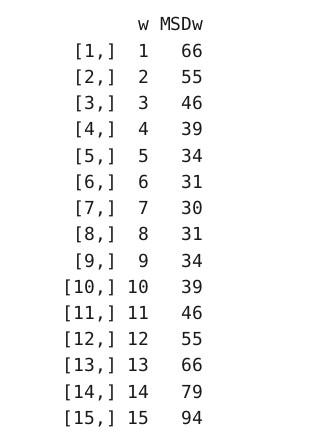
\includegraphics[width = 0.4\textwidth, keepaspectratio]{msdtable.jpeg} 
\end{center}
\end{frame}
%%%%%%%%%%%%%%%%%%%%%%%%%%%%%%%%%%%%%%%%%%%%%%%%%%%%%%%%%%%%

%%%%%%%%%%%%%%%%%%%%%%%%%%%%%%%%%%%%%%%%%%%%%%%%%%%%%%%%%%%%
\begin{frame}
%%%%%%%%%%%%%%%%%%%%%%%%%%%%%%%%%%%%%%%%%%%%%%%%%%%%%%%%%%%%

\frametitle{Behavior of MSD function}
Let's take the very simple dataset comprising of only 4 points 1, 3, 15 and 9.
\begin{center}
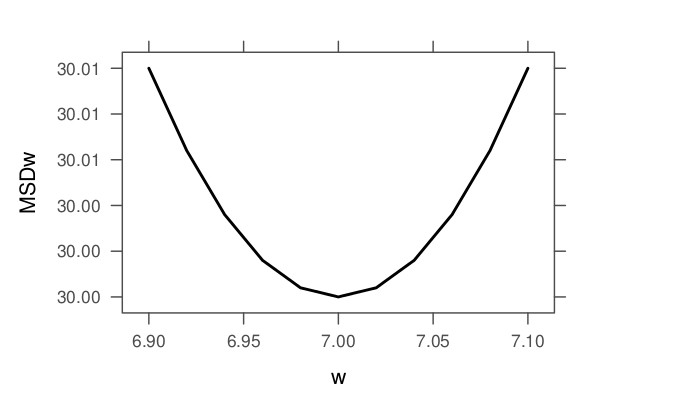
\includegraphics[width = 0.5\textwidth, keepaspectratio]{msdw.jpeg} 
\end{center}

\pause
\begin{center}
\item 7 is the mean !! \pause Can we prove it analytically as well?

\item We call MSD as this function evaluated at $\bar{x}$, i.e $$MSD= L_1(\bar{x})= \frac{1}{n}\sum_{i=1}^{n}(x_i-\bar{x})^2$$
\end{center}
\end{frame}
%%%%%%%%%%%%%%%%%%%%%%%%%%%%%%%%%%%%%%%%%%%%%%%%%%%%%%%%%%%%

%%%%%%%%%%%%%%%%%%%%%%%%%%%%%%%%%%%%%%%%%%%%%%%%%%%%%%%%%%%%
\begin{frame}
%%%%%%%%%%%%%%%%%%%%%%%%%%%%%%%%%%%%%%%%%%%%%%%%%%%%%%%%%%%%

\frametitle{Loss function}
\begin{itemize}
\item MSD function: $$L_1(w)=\frac{1}{n}\sum_{i=1}^{n} (x_i-w)^2$$ \\
\item MAD function: $$L_2(w)= \frac{1}{n}\sum_{i=1}^{n} |x_i-w|$$ \\

\item MAD stands for Mean Absolute Deviation
\item Minimize MSD function $\rightarrow$ Mean \pause
\item Minimize MAD function $\rightarrow$ Median \pause
\item Median is another measure of central tendency

\end{itemize}
\end{frame}
%%%%%%%%%%%%%%%%%%%%%%%%%%%%%%%%%%%%%%%%%%%%%%%%%%%%%%%%%%%%


%%%%%%%%%%%%%%%%%%%%%%%%%%%%%%%%%%%%%%%%%%%%%%%%%%%%%%%%%%%%
\begin{frame}
%%%%%%%%%%%%%%%%%%%%%%%%%%%%%%%%%%%%%%%%%%%%%%%%%%%%%%%%%%%%

\frametitle{Behavior of MAD}
Let's take the same dataset again 1, 3, 15 and 9.
\begin{center}
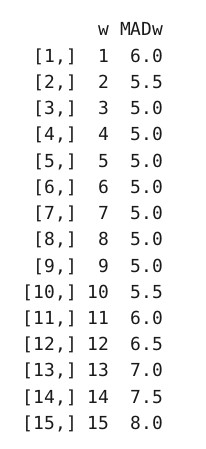
\includegraphics[width = 0.28\textwidth, keepaspectratio]{madtable.jpeg} 
\end{center}
\end{frame}
%%%%%%%%%%%%%%%%%%%%%%%%%%%%%%%%%%%%%%%%%%%%%%%%%%%%%%%%%%%%

%%%%%%%%%%%%%%%%%%%%%%%%%%%%%%%%%%%%%%%%%%%%%%%%%%%%%%%%%%%%
\begin{frame}
%%%%%%%%%%%%%%%%%%%%%%%%%%%%%%%%%%%%%%%%%%%%%%%%%%%%%%%%%%%%

\frametitle{Behavior of MAD}
Let's take the same dataset again 1, 3, 15 and 9.
\begin{center}
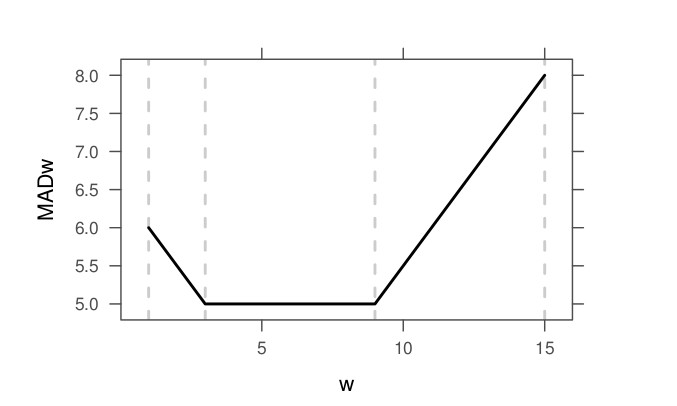
\includegraphics[width = 0.6\textwidth, keepaspectratio]{madw.jpeg} 
\end{center}

\pause
\begin{center}
Minimum attained at any point between 3 to 9. \pause All the points in [3,9] qualify as the median. \pause To keep it definite we will take (3+9)/2=6 as our median here.
\end{center}
\end{frame}
%%%%%%%%%%%%%%%%%%%%%%%%%%%%%%%%%%%%%%%%%%%%%%%%%%%%%%%%%%%%

%%%%%%%%%%%%%%%%%%%%%%%%%%%%%%%%%%%%%%%%%%%%%%%%%%%%%%%%%%%%
\begin{frame}
%%%%%%%%%%%%%%%%%%%%%%%%%%%%%%%%%%%%%%%%%%%%%%%%%%%%%%%%%%%%

\frametitle{Measures of Center: Median}
\textcolor{blue}{Definition} First order the data points $x_1, x_2, \cdots x_n$ in ascending order (including repetitions). Then \textbf{sample median} $\tilde{x}$ of the \emph{sample} $x_1, x_2, \cdots x_n$ is the single middle value of the \emph{ordered set} is $n$ is odd and the average of two middle values if $n$ is even.
\vspace{0.2in}
\begin{center}
Let's take an example.
\end{center}

\end{frame}
%%%%%%%%%%%%%%%%%%%%%%%%%%%%%%%%%%%%%%%%%%%%%%%%%%%%%%%%%%%%

%%%%%%%%%%%%%%%%%%%%%%%%%%%%%%%%%%%%%%%%%%%%%%%%%%%%%%%%%%%%
\begin{frame}
%%%%%%%%%%%%%%%%%%%%%%%%%%%%%%%%%%%%%%%%%%%%%%%%%%%%%%%%%%%%

\frametitle{Measures of Center: Median}
\textcolor{blue}{Example} Consider the following data set:\newline
$6.3, 10.2, 3.8, 7.9, 8.0, 5.5, 6.8$
\begin{itemize}
\item Number of observations? Odd or even? \pause \newline
      Ans. 7. Odd. \pause 
\item What's the next step? \pause \newline
      Ans. Order them. $3.8, 5.5, 6.3, 6.8, 7.9, 8.0, 10.2$ \pause
\item What is the middle position? What is the median? \pause \newline
      Ans. Middle position is 4. Median is 6.8

\end{itemize}

\end{frame}
%%%%%%%%%%%%%%%%%%%%%%%%%%%%%%%%%%%%%%%%%%%%%%%%%%%%%%%%%%%%

%%%%%%%%%%%%%%%%%%%%%%%%%%%%%%%%%%%%%%%%%%%%%%%%%%%%%%%%%%%%
\begin{frame}
%%%%%%%%%%%%%%%%%%%%%%%%%%%%%%%%%%%%%%%%%%%%%%%%%%%%%%%%%%%%
\frametitle{Measures of Center: Median}
\textcolor{blue}{Example} Now consider the following data set:\newline
$6.3, 10.2, 3.8, 7.9, 8.0, 5.5, 6.8, 7.3$
\begin{itemize}
\item Number of observations 8 which is even \pause

\item Order them from smallest to largest: $3.8, 5.5, 6.3, 6.8, 7.3, 7.9, 8.0, 10.2$\pause

\item What are the 2 middle positions? What is the median? \pause \newline
      Ans. Middle positions are 4 and 5. Median is $\tfrac{6.8 + 7.3}{2} =7.05$.
\end{itemize}

\end{frame}
%%%%%%%%%%%%%%%%%%%%%%%%%%%%%%%%%%%%%%%%%%%%%%%%%%%%%%%%%%%%

%%%%%%%%%%%%%%%%%%%%%%%%%%%%%%%%%%%%%%%%%%%%%%%%%%%%%%%%%%%%
\begin{frame}
%%%%%%%%%%%%%%%%%%%%%%%%%%%%%%%%%%%%%%%%%%%%%%%%%%%%%%%%%%%%
\frametitle{Measures of Center: Median}
So we can formulate the sample median $\tilde{x}$ as: 
\begin{itemize}
\item The $\big(\tfrac{n+1}{2}\big)$th ordered valued in the ordered list obtained from the sample when $n$ is odd.

\item The average of $\big(\tfrac{n}{2}\big)$th and $\big(\tfrac{n}{2} + 1\big)$th ordered values in the ordered list when $n$ is even.
\end{itemize}

\end{frame}
%%%%%%%%%%%%%%%%%%%%%%%%%%%%%%%%%%%%%%%%%%%%%%%%%%%%%%%%%%%%

%%%%%%%%%%%%%%%%%%%%%%%%%%%%%%%%%%%%%%%%%%%%%%%%%%%%%%%%%%%%
\begin{frame}[fragile]{Formulas for Sample Average, Variance, SD\;\;}
%%%%%%%%%%%%%%%%%%%%%%%%%%%%%%%%%%%%%%%%%%%%%%%%%%%%%%%%%%%%
\vspace{0.25cm}

$$\mbox{sample average } = \overline{x} = \mbox{ ``x-bar" }
= \frac{1}{n} \sum_{i=1}^n\, x_i$$

$$\mbox{sample variance } = s^2 = \mbox{ ``s-squared" }
= \frac{1}{n-1} \sum_{i=1}^n\, (x_i-\overline{x})^2$$

\begin{align*}
\mbox{sample standard deviation } &= s
= \sqrt{s^2} = \sqrt{\frac{1}{n-1} \sum_{i=1}^n\, (x_i-\overline{x})^2}\\
&= \mbox{ ``typical" distance from the average}
\end{align*}
\vskip0.1cm
Why divide by $(n-1)$ instead of $n$ for sample variance and SD?

\end{frame}
%%%%%%%%%%%%%%%%%%%%%%%%%%%%%%%%%%%%%%%%%%%%%%%%%%%%%%%%%%%%
\begin{frame}[allowframebreaks, fragile]{Why divide by $(n-1)$ for sample variance and SD?\;\;}
%%%%%%%%%%%%%%%%%%%%%%%%%%%%%%%%%%%%%%%%%%%%%%%%%%%%%%%%%%%%
\vspace{0.25cm}

\textbf{Variance} has a particular meaning in
statistics: \\
\textbf{mean squared distance from the average}
\begin{equation*}
MSD_n(\,\xbar\,)
= \frac{1}{n}\sum_{i=1}^n (x_i-\xbar)^2
%\label{eqn:MSDxbar}
\end{equation*}
Why collect data (\textbf{statistics})?  

To learn about the population (\textbf{parameters}).
\begin{equation*}
\text{population mean} = \mu = \text{``myoo"}
= \frac{1}{N}\sum_{i=1}^N x_i
%\label{eqn:mu}
\end{equation*}
\begin{equation*}
\text{popn variance} = \sigma^2 = \text{``sigma squared"}
= \frac{1}{N}\sum_{i=1}^N (x_i-\mu)^2
\end{equation*}

\newpage
%%%%%%%%%%%%%%%%%%%%%%%%%%
$\displaystyle{
\text{truth} = \text{popn variance}
= \sigma^2 = MSD_N(\,\mu\,) = \frac{1}{N}\sum_{i=1}^N (x_i-\mu)^2
}$
\vskip0.1cm

If we know the true popn mean ($\mu$)
and had a sample of $n$, use
\begin{equation}
\text{estimate}
= \sigmahat_{\mu}^2 = MSD_n(\,\mu\,) = \frac{1}{n}\sum_{i=1}^n (x_i-\mu)^2
\label{eqn:MSDmu}
\end{equation}
But, we almost never know $\mu$!  That's why we sample!
\begin{equation}
\text{realistic estimate}
= \sigmahat_{\xbar}^2 = MSD_n(\,\xbar\,) = \frac{1}{n}\sum_{i=1}^n (x_i-\xbar)^2
\label{eqn:MSDxbar}
\end{equation}
The problem: $\eqref{eqn:MSDxbar} \le \eqref{eqn:MSDmu}$.
\quad Why?\;\; ...and why is this a problem?\\
How does dividing by $(n-1)$ for \eqref{eqn:MSDxbar} help?
solve the problem?

\newpage
%%%%%%%%%%%%%%%%%%%%%%%%%%%%
OK. So, we should divide by a number smaller than $n$.

But, why $(n-1)$ in particular?
\vskip0.25cm

\textbf{Claim:}\;
Just $(n-1)$ observations and $\xbar$ are sufficient
to determine the one remaining observation.
\vskip0.25cm

\textbf{Proof:}\;
We know $n\xbar = x_1+x_2+\cdots +x_n$, since
$\xbar = \frac{1}{n} \sum x_i$

So, $x_n = n\xbar - (x_1+x_2+\cdots+x_{n-1})$.

\vskip0.4cm
In a sense, $\sum (x_i-\xbar)^2$  
adds up $(n-1)$ ``independent" values.
\vskip0.1cm

We say that the sum $\sum (x_i-\xbar)^2$
has $(n-1)$ \textbf{degrees of freedom} .
\vskip0.1cm

So, the sample average squared deviation (variance) is defined as
\vskip0.4cm

$\displaystyle{
s^2 = \mbox{ ``s-squared" }
= \frac{1}{n-1} \sum_{i=1}^n\, (x_i-\overline{x})^2
}$

\end{frame}





%%%%%%%%%%%%%%%%%%%%%%%%%%%%%%%%%%%%%%%%%%%%%%%%%%%%%%%%%%%%
\begin{frame}[allowframebreaks, fragile]{Linear Transformation of Data\;\;}
%%%%%%%%%%%%%%%%%%%%%%%%%%%%%%%%%%%%%%%%%%%%%%%%%%%%%%%%%%%%
\vspace{0.25cm}
Sometimes we want to analyze data in different units \newline

Temperature unit in USA :  degree Fahrenheit \newline
Temperature unit in India: degree Celsius \newline

Temperature: 
$\displaystyle{ \text{Celsius} = \frac{5}{9} (\text{Fahrenheit} - 32)}$  

Temperature: 
$\displaystyle{ \text{Celsius}  = -\left(\frac{160}{9}\right) + \left(\frac{5}{9}\right)\text{Fahrenheit}}$
\newpage
%%%%%%%%%%%%%%%%%%%%%%%%%%%
High temperature in Chicago last 5 days of December
\begin{knitrout}\small
\definecolor{shadecolor}{rgb}{1, 1, 1}\color{fgcolor}\begin{kframe}
\begin{alltt}
\hlstd{Fahrenheit} \hlkwb{<-} \hlkwd{c}\hlstd{(}\hlnum{39}\hlstd{,} \hlnum{39}\hlstd{,} \hlnum{29}\hlstd{,} \hlnum{28}\hlstd{,} \hlnum{31}\hlstd{)}
\hlstd{OLD} \hlkwb{<-} \hlkwd{options}\hlstd{(}\hlkwc{digits}\hlstd{=}\hlnum{3}\hlstd{)}

\hlstd{Fahrenheit}
\end{alltt}
\begin{verbatim}
[1] 39 39 29 28 31
\end{verbatim}
\begin{alltt}
\hlkwd{mean}\hlstd{(Fahrenheit)}
\end{alltt}
\begin{verbatim}
[1] 33.2
\end{verbatim}
\end{kframe}
\end{knitrout}

%%%%%%%%%%%%%%%%%%%%%%%%%%%

\begin{knitrout}\small
\definecolor{shadecolor}{rgb}{1, 1, 1}\color{fgcolor}\begin{kframe}
\begin{alltt}
\hlstd{Celsius} \hlkwb{=} \hlopt{-}\hlstd{(}\hlnum{160}\hlopt{/}\hlnum{9}\hlstd{)} \hlopt{+} \hlstd{(}\hlnum{5}\hlopt{/}\hlnum{9}\hlstd{)}\hlopt{*}\hlstd{Fahrenheit}

\hlkwd{rbind}\hlstd{(Fahrenheit, Celsius)}
\end{alltt}
\begin{verbatim}
            [,1]  [,2]  [,3]  [,4]   [,5]
Fahrenheit 39.00 39.00 29.00 28.00 31.000
Celsius     3.89  3.89 -1.67 -2.22 -0.556
\end{verbatim}
\begin{alltt}
\hlkwd{mean}\hlstd{(Celsius)}
\end{alltt}
\begin{verbatim}
[1] 0.667
\end{verbatim}
\begin{alltt}
\hlkwd{mean}\hlstd{(Celsius)}
\end{alltt}
\begin{verbatim}
[1] 0.667
\end{verbatim}
\begin{alltt}
\hlopt{-}\hlstd{(}\hlnum{160}\hlopt{/}\hlnum{9}\hlstd{)} \hlopt{+} \hlstd{(}\hlnum{5}\hlopt{/}\hlnum{9}\hlstd{)} \hlopt{*} \hlkwd{mean}\hlstd{(Fahrenheit)}
\end{alltt}
\begin{verbatim}
[1] 0.667
\end{verbatim}
\end{kframe}
\end{knitrout}


\textbf{Claim:} \;
If data $x_1, x_2,\ldots, x_n$ \\
are
linearly transformed to
$y_i = a + b x_i$
\vskip0.2cm

Then, $\ybar = a + b\xbar$.
\vskip0.5cm

\textbf{Proof:}\;

A proof appears in Section 1.4 (Math Supplement).

\newpage
%%%%%%%%%%%%%%%%%%%%%%%%%%%
\begin{knitrout}\small
\definecolor{shadecolor}{rgb}{1, 1, 1}\color{fgcolor}\begin{kframe}
\begin{alltt}
\hlkwd{sd}\hlstd{(Celsius)}
\end{alltt}
\begin{verbatim}
[1] 3
\end{verbatim}
\begin{alltt}
\hlstd{(}\hlnum{5}\hlopt{/}\hlnum{9}\hlstd{)} \hlopt{*} \hlkwd{sd}\hlstd{(Fahrenheit)}
\end{alltt}
\begin{verbatim}
[1] 3
\end{verbatim}
\end{kframe}
\end{knitrout}

\textbf{Claim:} \;
If data $x_1, x_2,\ldots, x_n$ \\
are
linearly transformed to
$y_i = a + b x_i$
\vskip0.2cm

Then, $SD(y) = s_y = |b|s_x = |b|SD(x)$.
\vskip0.5cm

\textbf{Proof:}\;
On your own for HW \#2.



\end{frame}

\begin{frame}[allowframebreaks, fragile]{The distribution of retweets\;\;}
\begin{knitrout}\small
\definecolor{shadecolor}{rgb}{1, 1, 1}\color{fgcolor}

{\centering 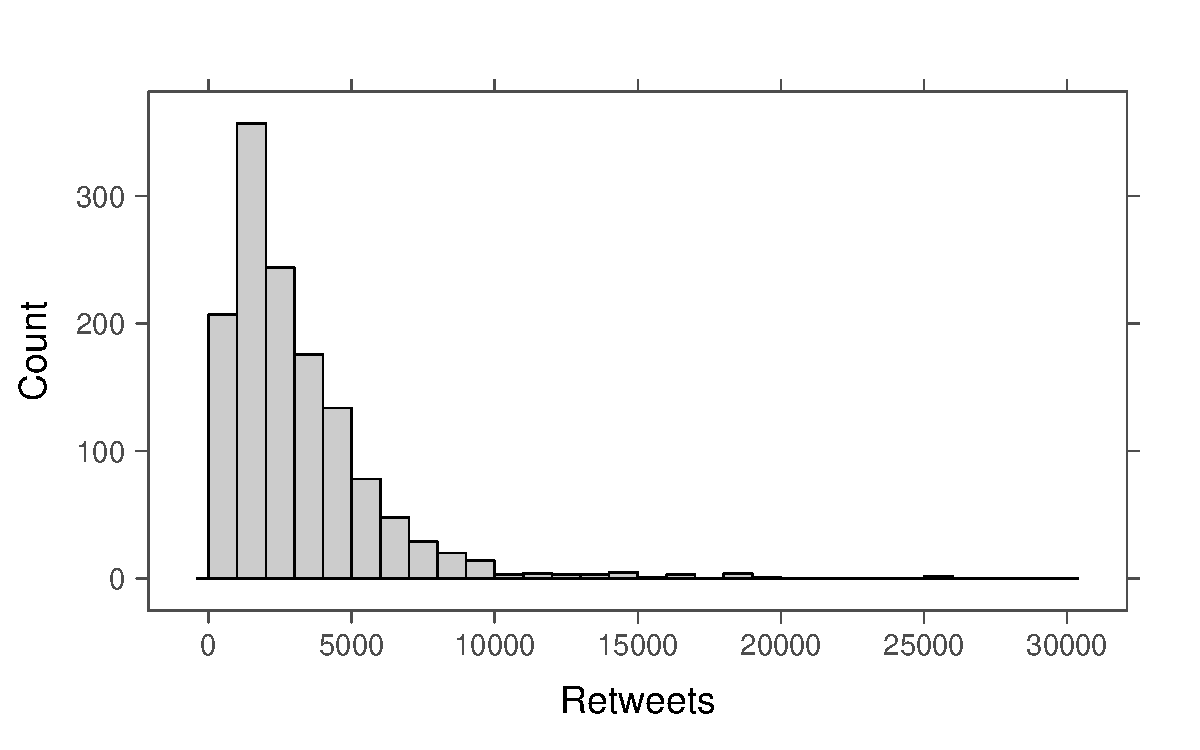
\includegraphics[width=0.89\linewidth]{figure/graphics-unnamed-chunk-5-1} 

}



\end{knitrout}

\newpage
\begin{knitrout}\small
\definecolor{shadecolor}{rgb}{1, 1, 1}\color{fgcolor}

{\centering 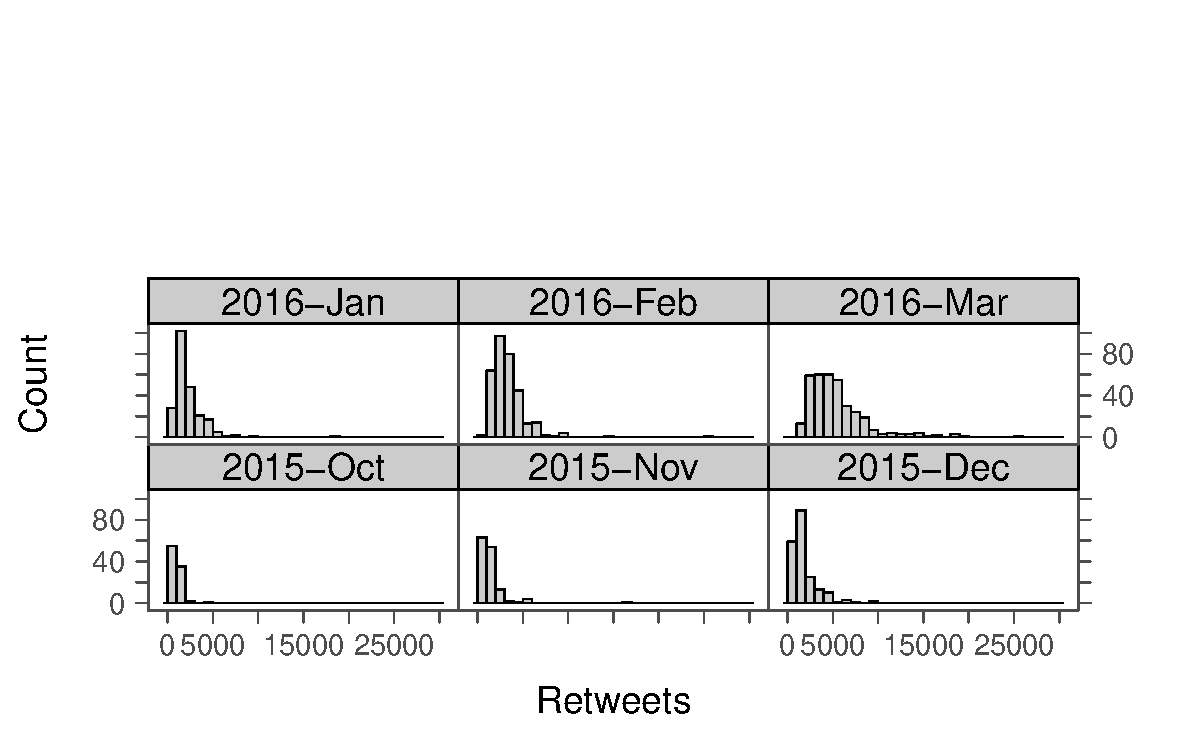
\includegraphics[width=1\linewidth]{figure/graphics-unnamed-chunk-6-1} 

}



\end{knitrout}

\newpage
Let's make the comparison based on percentages, not counts
\begin{knitrout}\small
\definecolor{shadecolor}{rgb}{1, 1, 1}\color{fgcolor}

{\centering 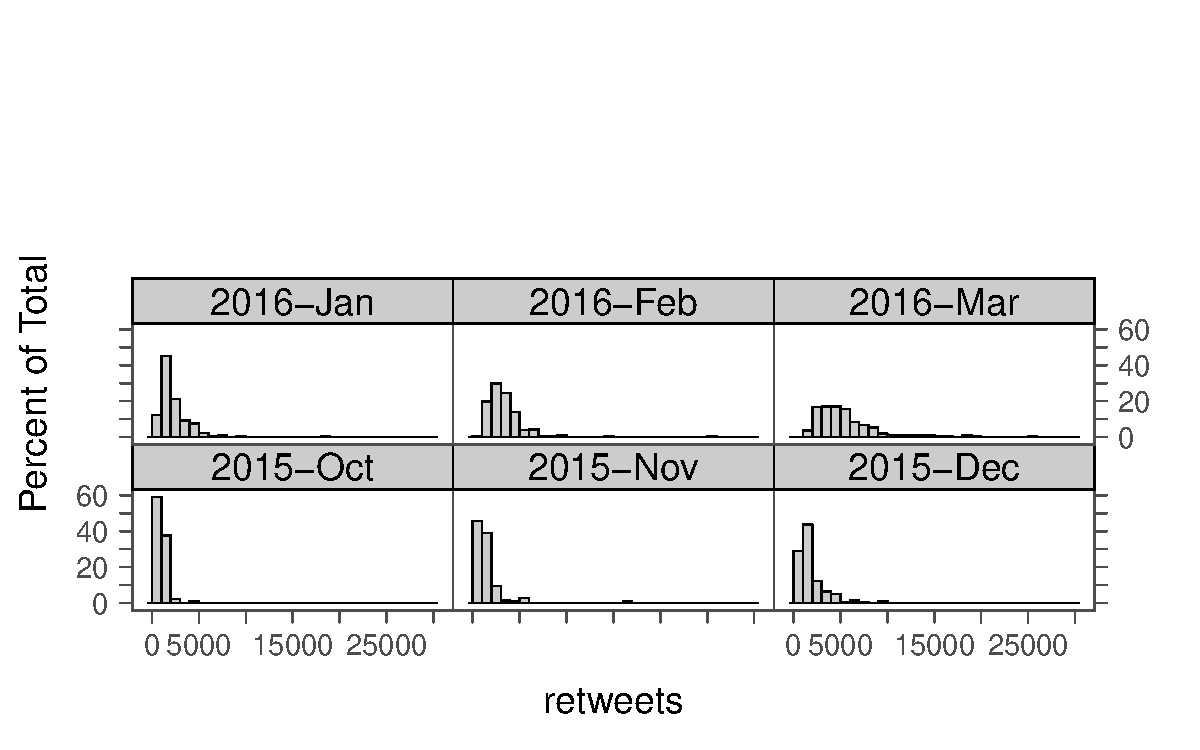
\includegraphics[width=1\linewidth]{figure/graphics-unnamed-chunk-7-1} 

}



\end{knitrout}
\end{frame}

\begin{frame}[allowframebreaks, fragile]{The distribution of logarithm of retweets\;\;}
\begin{knitrout}\small
\definecolor{shadecolor}{rgb}{1, 1, 1}\color{fgcolor}

{\centering 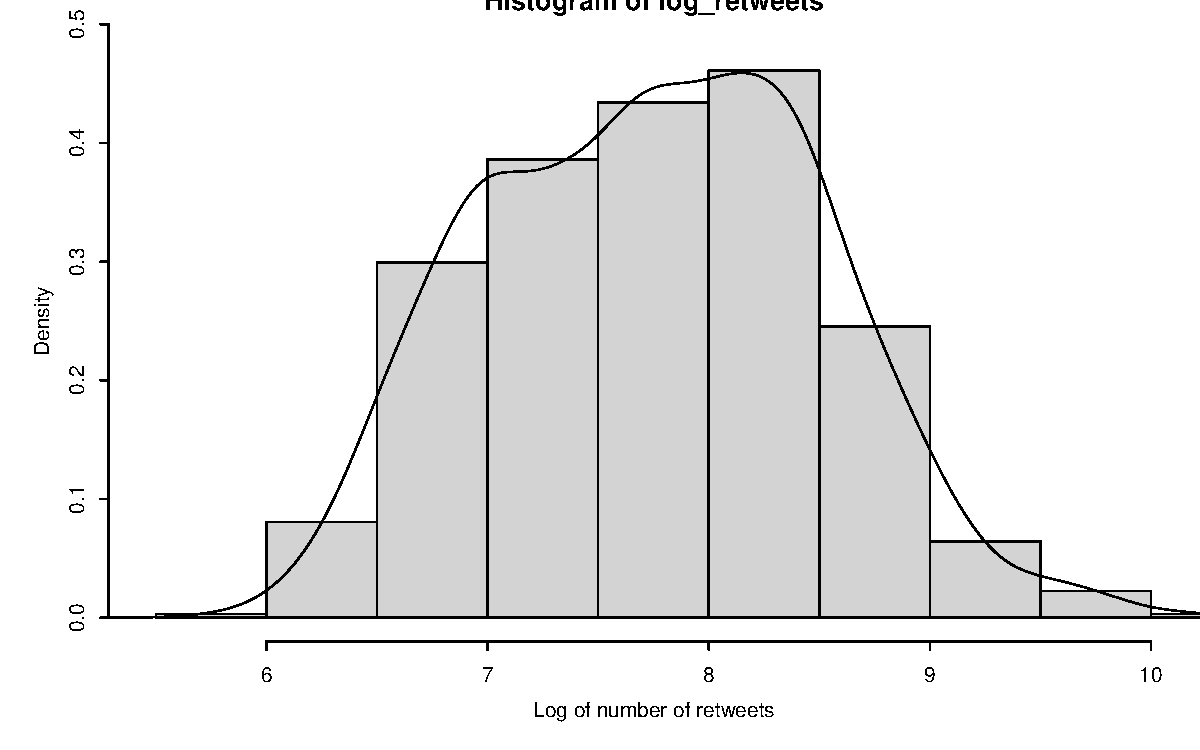
\includegraphics[width=0.89\linewidth]{figure/graphics-unnamed-chunk-8-1} 

}



\end{knitrout}

\begin{knitrout}\small
\definecolor{shadecolor}{rgb}{1, 1, 1}\color{fgcolor}

{\centering 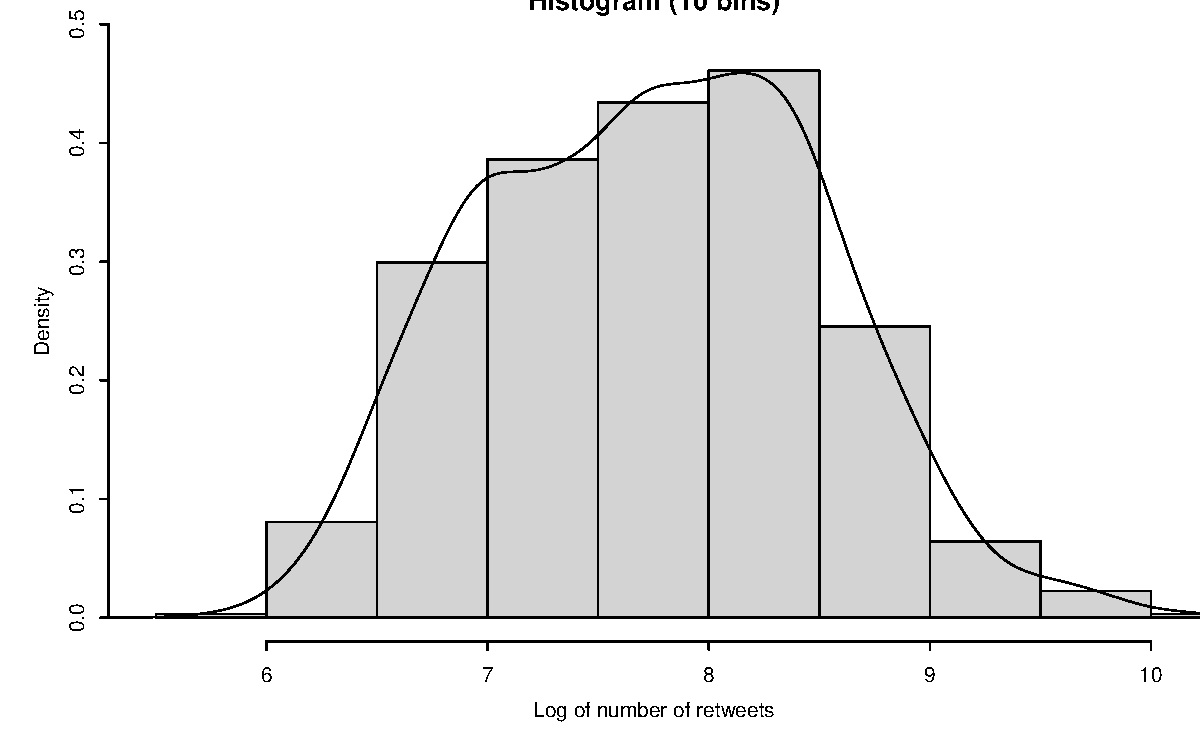
\includegraphics[width=0.89\linewidth]{figure/graphics-unnamed-chunk-9-1} 

}



\end{knitrout}

\begin{knitrout}\small
\definecolor{shadecolor}{rgb}{1, 1, 1}\color{fgcolor}

{\centering 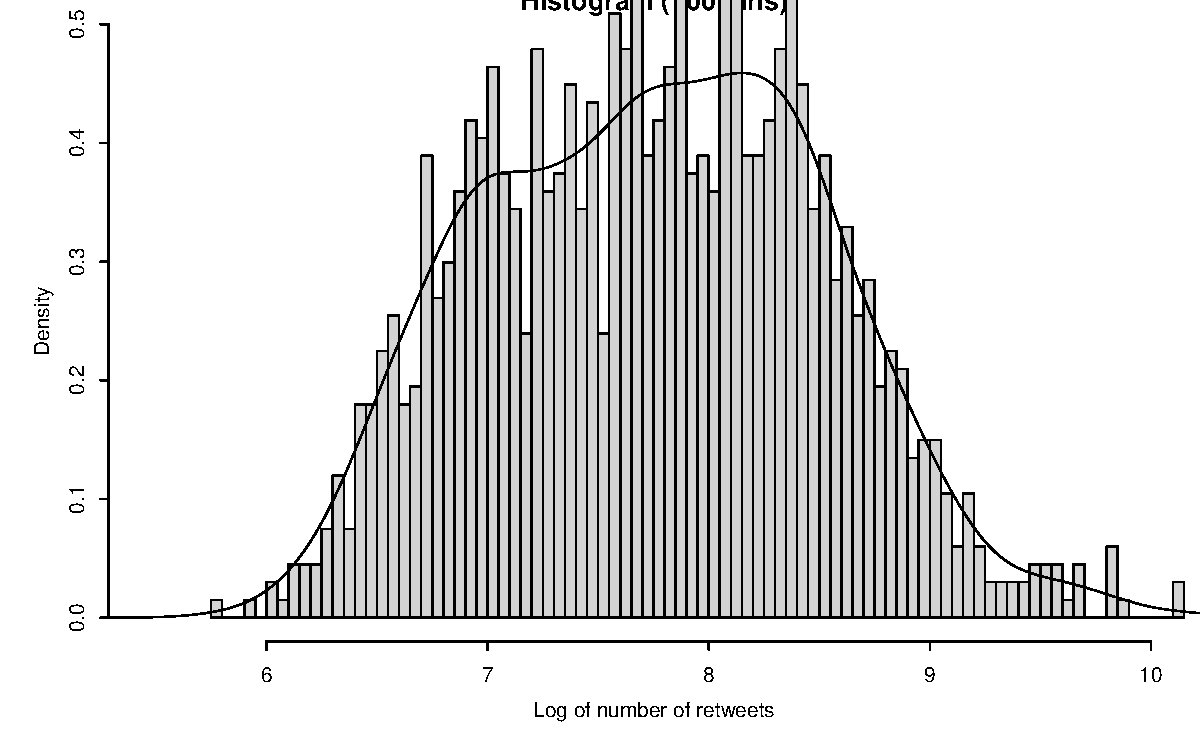
\includegraphics[width=0.89\linewidth]{figure/graphics-unnamed-chunk-10-1} 

}



\end{knitrout}

\begin{knitrout}\small
\definecolor{shadecolor}{rgb}{1, 1, 1}\color{fgcolor}

{\centering 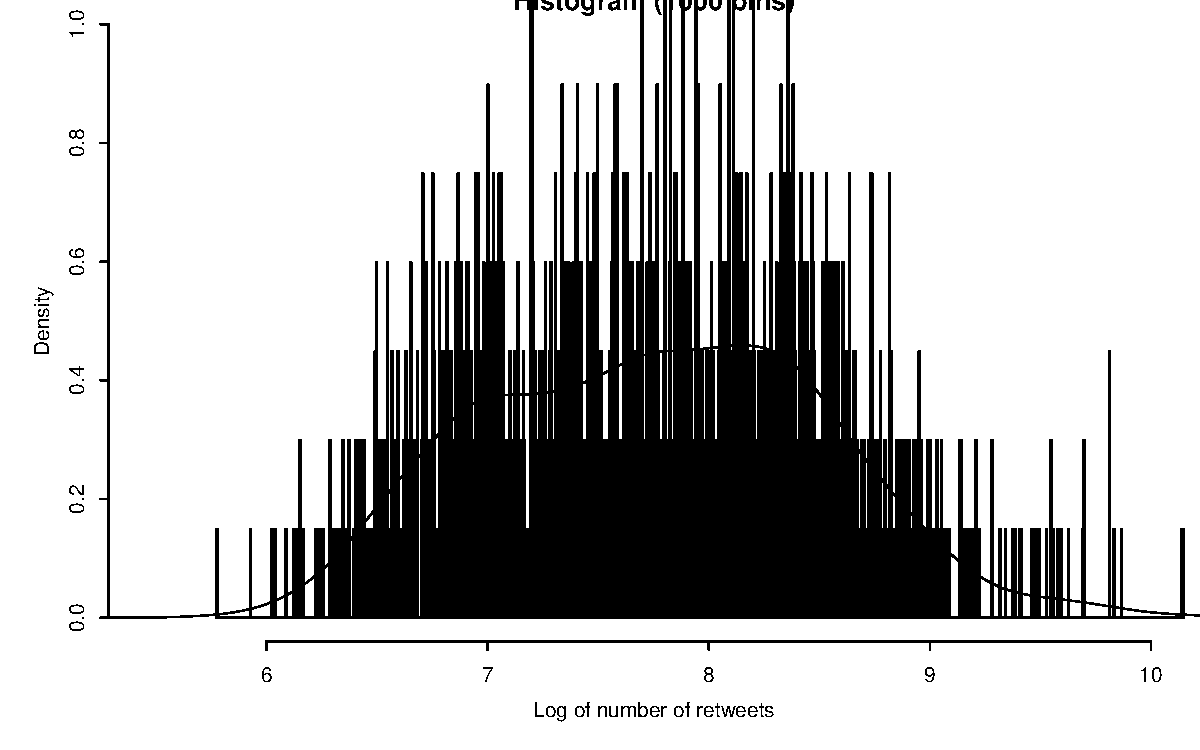
\includegraphics[width=0.89\linewidth]{figure/graphics-unnamed-chunk-11-1} 

}



\end{knitrout}

\begin{knitrout}\small
\definecolor{shadecolor}{rgb}{1, 1, 1}\color{fgcolor}

{\centering 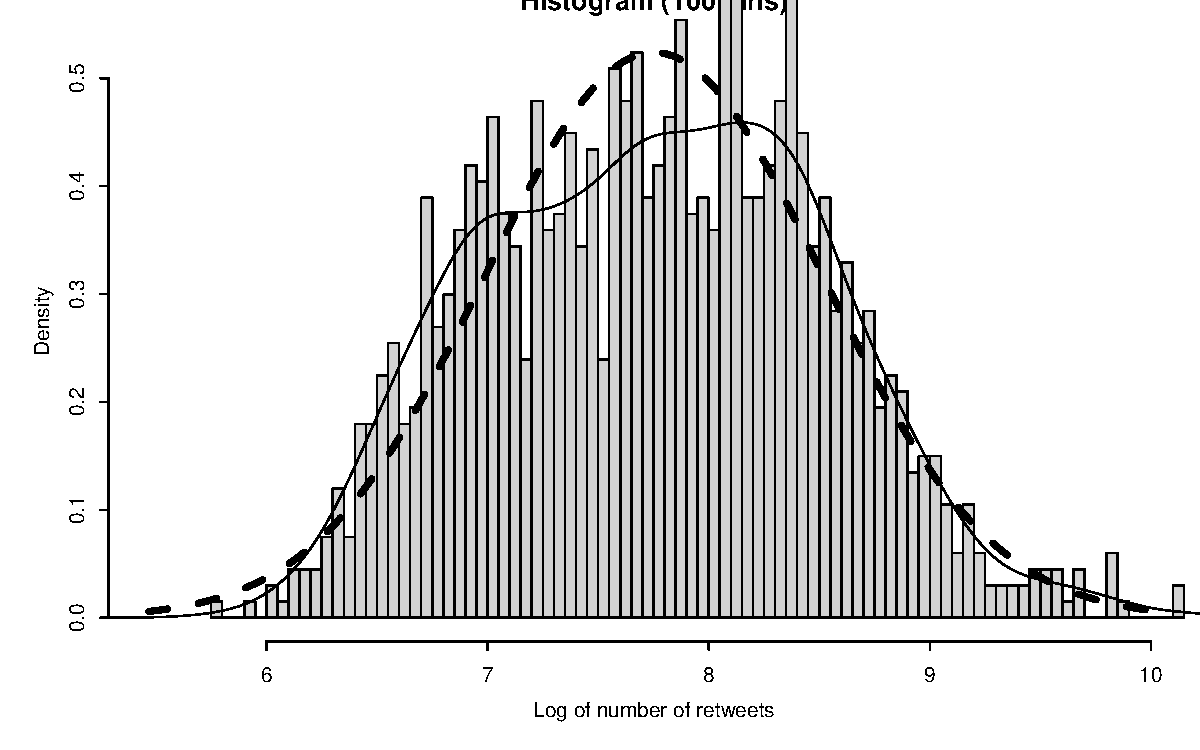
\includegraphics[width=0.89\linewidth]{figure/graphics-unnamed-chunk-12-1} 

}



\end{knitrout}
\newpage
\end{frame}

%%%%%%%%%%%%%%%%%%%%%%%%%%%
\begin{frame}[fragile]
%%%%%%%%%%%%%%%%%%%%%%%%%%%

\frametitle{Normal Distribution}
\begin{center}
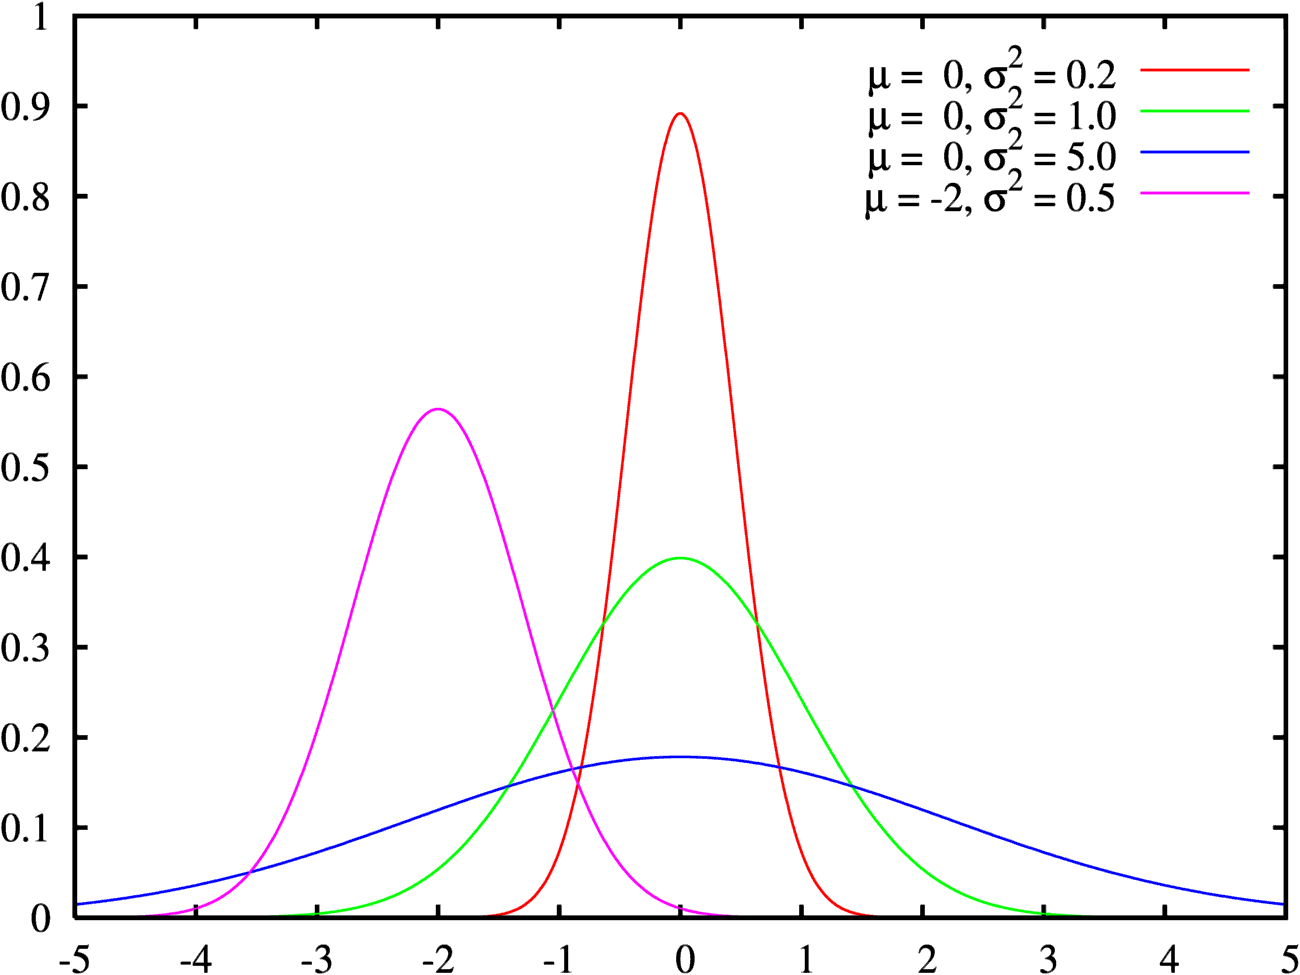
\includegraphics[width=7cm,keepaspectratio]{Normal_distribution.png} 
\end{center}
\end{frame}
%%%%%%%%%%%%%%%%%%%%%%%%%%%

%%%%%%%%%%%%%%%%%%%%%%%%%%%
\begin{frame}[fragile]
%%%%%%%%%%%%%%%%%%%%%%%%%%%

\frametitle{ Facts about Normal Distribution}
\begin{itemize}
\item Two parameters. Mean ($\mu$) and standard deviation ($\sigma$) \pause
\item $\mu$ and $\sigma$ are population parameters. \pause
\item $\mu=0$ and $\sigma=1$ refers to the standard normal distribution. \pause
\item Centred around $\mu$.
\item For standard normal $$ P( X>1) = P( X <-1) $$ Why? 
\item The formula for $N(\mu, \sigma)$ is (don't be scared - just FYI!)
$$f(x) = \frac{1}{\sqrt{2\pi}\sigma}e^{-\frac{(x-\mu)^2}{2\sigma^2}} $$
\end{itemize}
\end{frame}
%%%%%%%%%%%%%%%%%%%%%%%%%%%


%%%%%%%%%%%%%%%%%%%%%%%%%%%
\begin{frame}[fragile]
%%%%%%%%%%%%%%%%%%%%%%%%%%%

\frametitle{Properties of Normal distribution}
 For a  Normal Distribution ( mean $\mu=0$ and sd $\sigma=1$)
\begin{center}
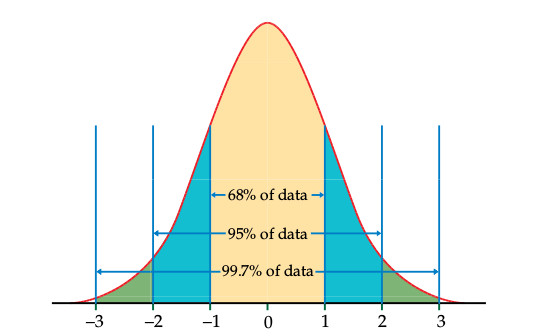
\includegraphics[width=7cm,keepaspectratio]{6895997.jpeg} 
\end{center}

This is called the $68 \%- 95 \% - 99.7 \% $ rule. This often simplifies our calculations.

What happens for a general $\mu$ and $\sigma$?

\end{frame}
%%%%%%%%%%%%%%%%%%%%%%%%%%%



%%%%%%%%%%%%%%%%%%%%%%%%%%%
\begin{frame}
%%%%%%%%%%%%%%%%%%%%%%%%%%%

\frametitle{Properties of Normal distribution}
 For a Normal Distribution ( $\mu=1000$ and $\sigma=100$)
\begin{center}
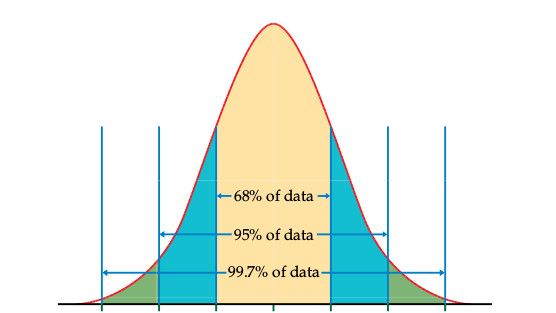
\includegraphics[width=7cm,keepaspectratio]{generalnormal6895997.jpeg} 
\end{center}
\begin{center}
\tiny{700 \hspace{0.09 in}  800  \hspace{0.09 in}    900  \hspace{0.09 in}   1000  \hspace{0.06 in}   1100   \hspace{0.06 in}  1200 \hspace{0.06 in}    1300 }
\end{center}

\begin{center}
\tiny{$\mu-3\sigma$ \hspace{0.03 in}  $\mu-2\sigma$  \hspace{0.03 in}    $\mu-\sigma$  \hspace{0.03 in}   $\mu$  \hspace{0.03 in}   $\mu+\sigma$   \hspace{0.03 in}  $\mu+2\sigma$ \hspace{0.03 in}    $\mu+3\sigma$ }


\end{center}
\end{frame}
%%%%%%%%%%%%%%%%%%%%%%%%%%%

%%%%%%%%%%%%%%%%%%%%%%%%%%%
\begin{frame}{Cumulative Proportions and Standard Normal Table}
%%%%%%%%%%%%%%%%%%%%%%%%%%%

\begin{itemize}
\item \textbf{Cumulative proportions}: The proportion of observations in a distribution that lie at or below a given value $x$.
\item For $N(0,1)$, use the standard normal table (Table A in textbook) to calculate cumulative proportions for $x$.
\end{itemize}
\begin{center}
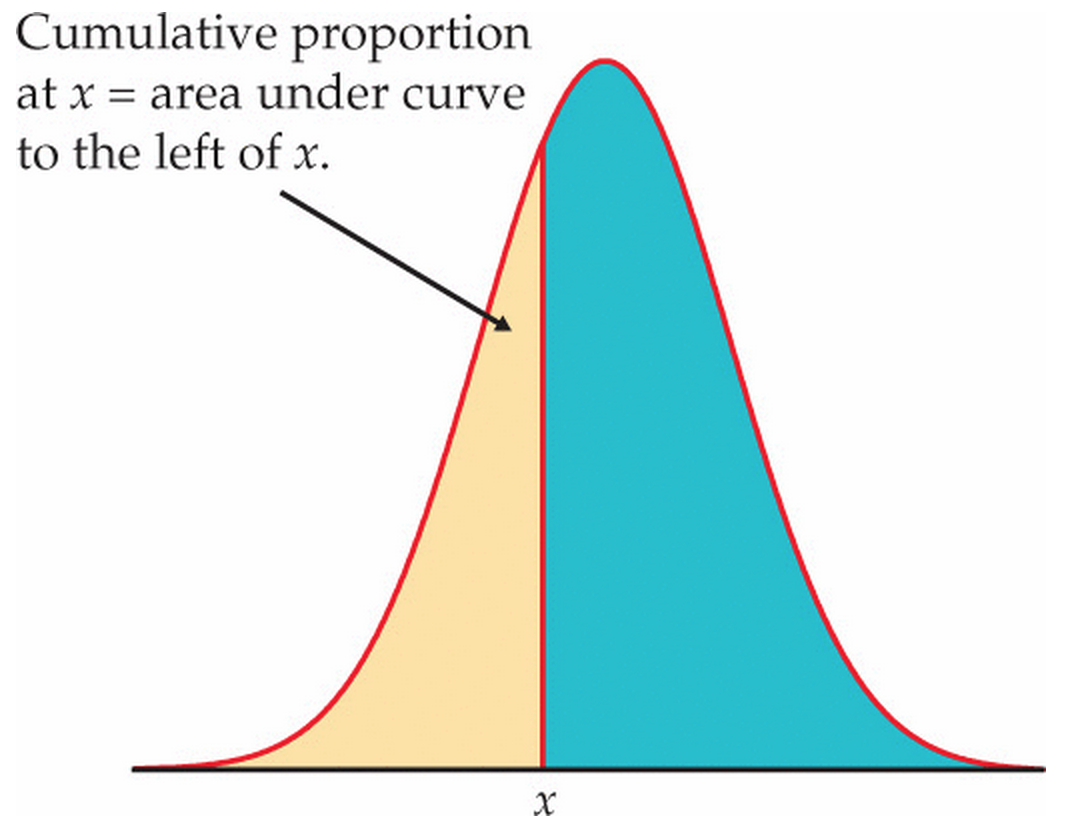
\includegraphics[height=2in]{P10.png}
\end{center}
\end{frame}
%%%%%%%%%%%%%%%%%%%%%%%%%%%


%%%%%%%%%%%%%%%%%%%%%%%%%%%
\begin{frame}{Cumulative Proportions and Standard Normal Table}
%%%%%%%%%%%%%%%%%%%%%%%%%%%

For $N(0,1)$, we can calculate all of the following areas using cumulative proportions:
\begin{center}
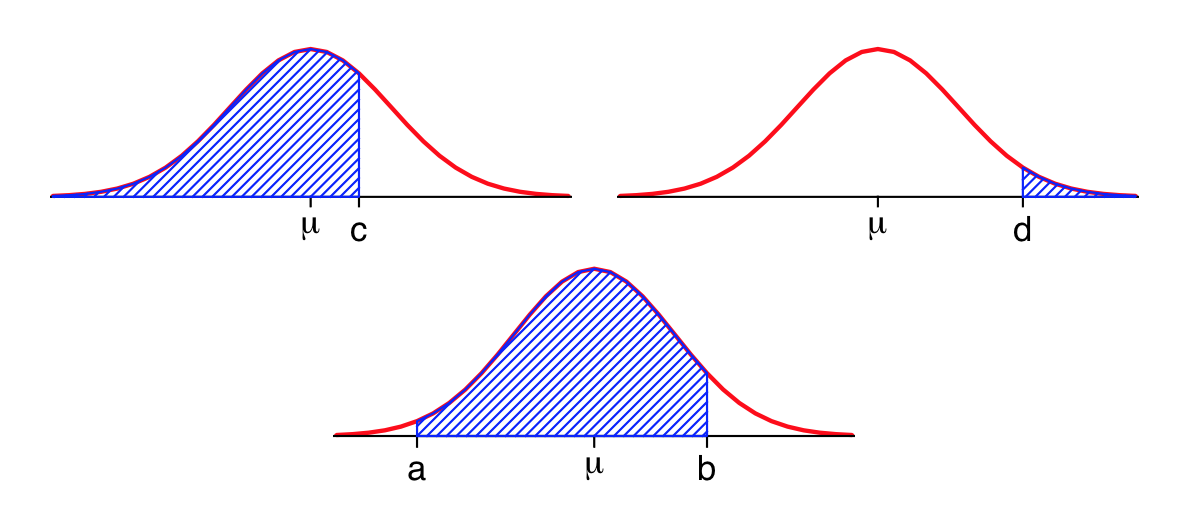
\includegraphics[height=1.8in]{P9.png}
\end{center}
\end{frame}
%%%%%%%%%%%%%%%%%%%%%%%%%%%

%%%%%%%%%%%%%%%%%%%%%%%%%%%
\begin{frame}
%%%%%%%%%%%%%%%%%%%%%%%%%%%

\frametitle{Normal Distribution}
\begin{itemize}
\item Many sets of data follow normal distribution. \pause
\item It is a symmetric, bell-curved distribution and has many nice properties ! \pause
\item A lot of statistical methodologies are based on the properties of this distribution. \pause
\item Naturally, there is a tendency to use it everywhere we can even though the data is not actually coming from a normal distribution. \pause
\item We should start by comparing the data with normal distribution. \pause
\end{itemize}
\end{frame}
%%%%%%%%%%%%%%%%%%%%%%%%%%%

%%%%%%%%%%%%%%%%%%%%%%%%%%%
\begin{frame}
%%%%%%%%%%%%%%%%%%%%%%%%%%%

\frametitle{Standardization and z-score }
\begin{itemize}

\item If $x$ is an observation from a distribution with mean (Population mean) $\mu$ and standard deviation $\sigma$ then , the standardized value is 
$$z=\frac{x-\mu}{\sigma}$$ \pause 

\item This is also called the $z-score$. \pause
\item Example?\pause   Assume that, time spent on the calls ( The data from Lecture 1 ) follows approximately a normal distribution with mean $\mu= 1000$ and $\sigma=100$. \pause
\item Suppose on particular observation is 870, $$z-\text{score}= \frac{670-1000}{100}= -1.3$$
\item We will use this z-score later to make some conclusions.
\end{itemize}
\end{frame}
%%%%%%%%%%%%%%%%%%%%%%%%%%%




\begin{frame}[allowframebreaks, fragile]{The normal density model in R\;\;}

The "normal density" model.  \newline

A good fit for these data distributions? \newline

A numerical look \newline 

What percent of area under standard normal density is above/below 1?
\begin{knitrout}\small
\definecolor{shadecolor}{rgb}{1, 1, 1}\color{fgcolor}\begin{kframe}
\begin{alltt}
\hlkwd{pnorm}\hlstd{(}\hlopt{-}\hlnum{1}\hlstd{,} \hlkwc{m}\hlstd{=}\hlnum{0}\hlstd{,} \hlkwc{s}\hlstd{=}\hlnum{1}\hlstd{)}
\end{alltt}
\begin{verbatim}
[1] 0.1587
\end{verbatim}
\begin{alltt}
\hlkwd{pnorm}\hlstd{(}\hlopt{-}\hlnum{1}\hlstd{)}
\end{alltt}
\begin{verbatim}
[1] 0.1587
\end{verbatim}
\begin{alltt}
\hlnum{1} \hlopt{-} \hlkwd{pnorm}\hlstd{(}\hlnum{1}\hlstd{)}
\end{alltt}
\begin{verbatim}
[1] 0.1587
\end{verbatim}
\end{kframe}
\end{knitrout}
\newpage

What percent of area under \emph{any} normal density is above/below 1 sd from mean?
\begin{knitrout}\small
\definecolor{shadecolor}{rgb}{1, 1, 1}\color{fgcolor}\begin{kframe}
\begin{alltt}
\hlstd{mtweets} \hlkwb{<-} \hlkwd{mean}\hlstd{(log_retweets)}
\hlstd{mtweets}
\end{alltt}
\begin{verbatim}
[1] 7.753
\end{verbatim}
\begin{alltt}
\hlstd{stweets} \hlkwb{<-} \hlkwd{sd}\hlstd{(log_retweets)}
\hlstd{stweets}
\end{alltt}
\begin{verbatim}
[1] 0.7613
\end{verbatim}
\begin{alltt}
\hlnum{1} \hlopt{-} \hlkwd{pnorm}\hlstd{(mtweets} \hlopt{+} \hlstd{stweets,} \hlkwc{m}\hlstd{=mtweets,} \hlkwc{s}\hlstd{=stweets)}
\end{alltt}
\begin{verbatim}
[1] 0.1587
\end{verbatim}
\begin{alltt}
\hlkwd{pnorm}\hlstd{(mtweets} \hlopt{-} \hlstd{stweets,} \hlkwc{m}\hlstd{=mtweets,} \hlkwc{s}\hlstd{=stweets)}
\end{alltt}
\begin{verbatim}
[1] 0.1587
\end{verbatim}
\end{kframe}
\end{knitrout}
\newpage

What percent of the observed data are right/left of 1 sd from mean?


\begin{knitrout}\small
\definecolor{shadecolor}{rgb}{1, 1, 1}\color{fgcolor}\begin{kframe}
\begin{alltt}
\hlkwd{sum}\hlstd{(log_retweets} \hlopt{>=} \hlstd{mtweets} \hlopt{+} \hlstd{stweets,} \hlkwc{na.rm}\hlstd{=}\hlnum{TRUE}\hlstd{)} \hlopt{/} \hlstd{n}
\end{alltt}
\begin{verbatim}
[1] 0.1639
\end{verbatim}
\begin{alltt}
\hlkwd{sum}\hlstd{(log_retweets} \hlopt{<=} \hlstd{mtweets} \hlopt{-} \hlstd{stweets,} \hlkwc{na.rm}\hlstd{=}\hlnum{TRUE}\hlstd{)} \hlopt{/} \hlstd{n}
\end{alltt}
\begin{verbatim}
[1] 0.1886
\end{verbatim}
\end{kframe}
\end{knitrout}
\newpage

What percent of the model/data are 2 sd to the right mean?
\begin{knitrout}\small
\definecolor{shadecolor}{rgb}{1, 1, 1}\color{fgcolor}\begin{kframe}
\begin{alltt}
\hlnum{1} \hlopt{-} \hlkwd{pnorm}\hlstd{(}\hlnum{2}\hlstd{)}
\end{alltt}
\begin{verbatim}
[1] 0.02275
\end{verbatim}
\begin{alltt}
\hlkwd{sum}\hlstd{(log_retweets} \hlopt{>=} \hlstd{mtweets} \hlopt{+} \hlnum{2}\hlopt{*}\hlstd{stweets,} \hlkwc{na.rm}\hlstd{=}\hlnum{TRUE}\hlstd{)} \hlopt{/} \hlstd{n}
\end{alltt}
\begin{verbatim}
[1] 0.02096
\end{verbatim}
\end{kframe}
\end{knitrout}

What percent of the model/data are 2 sd to the left of mean?
\begin{knitrout}\small
\definecolor{shadecolor}{rgb}{1, 1, 1}\color{fgcolor}\begin{kframe}
\begin{alltt}
\hlkwd{pnorm}\hlstd{(}\hlopt{-}\hlnum{2}\hlstd{)}
\hlkwd{sum}\hlstd{(log_retweets} \hlopt{<=} \hlstd{mtweets} \hlopt{-} \hlnum{2}\hlopt{*}\hlstd{stweets,} \hlkwc{na.rm}\hlstd{=}\hlnum{TRUE}\hlstd{)} \hlopt{/} \hlstd{n}
\end{alltt}
\end{kframe}
\end{knitrout}

\end{frame}

%%%%%%%%%%%%%%%%%%%%%%%%%%%%%%%%%%%%%%%%%%%
\begin{frame}
%%%%%%%%%%%%%%%%%%%%%%%%%%%%%%%%%%%%%%%%%%%
\frametitle{When things are not normal!!}
\begin{knitrout}\small
\definecolor{shadecolor}{rgb}{1, 1, 1}\color{fgcolor}

{\centering 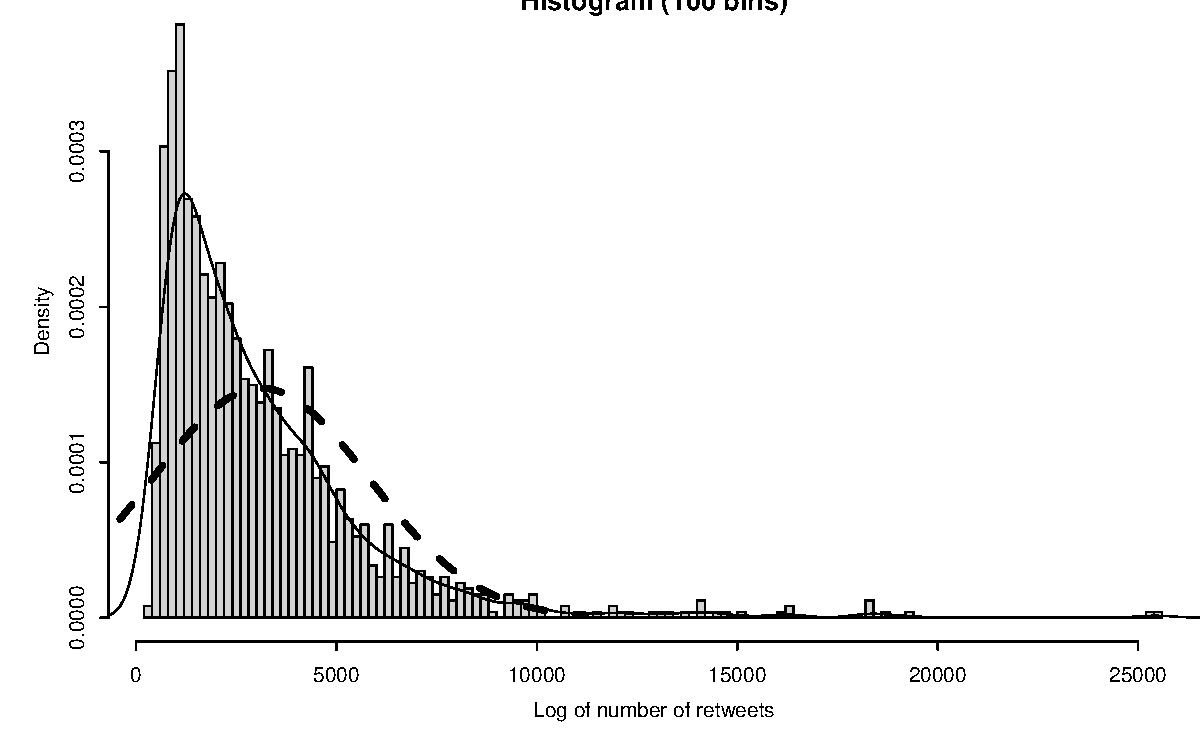
\includegraphics[width=0.89\linewidth]{figure/graphics-unnamed-chunk-18-1} 

}



\end{knitrout}
\end{frame}

%%%%%%%%%%%%%%%%%%%%%%%%%%%%%%%%%%%%%%%%%%%
\begin{frame}
%%%%%%%%%%%%%%%%%%%%%%%%%%%%%%%%%%%%%%%%%%%
\frametitle{Skewness}
\begin{center}
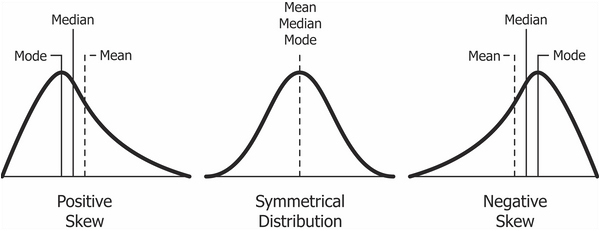
\includegraphics[width=7cm,keepaspectratio]{skewness.jpg} 
\end{center}
\end{frame}

%%%%%%%%%%%%%%%%%%%%%%%%%%%%%%%%%%%%%%%%%%%
\begin{frame}[fragile]
%%%%%%%%%%%%%%%%%%%%%%%%%%%%%%%%%%%%%%%%%%%
\frametitle{A Step back: Quantiles}

\begin{itemize}
\item The \emph{k} th quantile of a set of values divides them so that $100*k$  
of the values lie below and $100*(1-k)$ of the values lie above. \pause \newline

\item the $0.25$th quantile is known first/lower quartile ($Q_1$)  \pause \newline

\item the $0.50$th quantile is known as median ($Q_2$) \pause \newline

\item the $0.75$th quantile is known as third/upper quartile ($Q_3$) \pause \newline

\end{itemize}
\end{frame}
%%%%%%%%%%%%%%%%%%%%%%%%%%%%%%%%%%%%%%%%%%%


%%%%%%%%%%%%%%%%%%%%%%%%%%%%%%%%%%%%%%%%%%%
\begin{frame}[fragile]
%%%%%%%%%%%%%%%%%%%%%%%%%%%%%%%%%%%%%%%%%%%
\frametitle{A Step back: Quantiles}

Lets look at the quantiles of a set of values - $3.4, 2.3, 6.7, 2.1, 5.0$ \pause \newline

First sort the values in order
$$ 2.1, \; \; 2.3 \; \; 3.4 \;\; 5.0 \;\; 6.7 $$

Then the quantiles for this data is given as follows 

\begin{tabular}{|c|c|c|c|c|c|}
\hline
Sample fraction & 0 & 0.25 & 0.50 & 0.75 & 1 \\ \hline
Quantiles & 2.1 & 2.3 & 3.4 & 5.0 & 6.7 \\ \hline
\end{tabular}
\end{frame}
%%%%%%%%%%%%%%%%%%%%%%%%%%%%%%%%%%%%%%%%%%%

%%%%%%%%%%%%%%%%%%%%%%%%%%%%%%%%%%%%%%%%%%%
\begin{frame}[fragile]
%%%%%%%%%%%%%%%%%%%%%%%%%%%%%%%%%%%%%%%%%%%
\frametitle{Quantiles in R}

\begin{knitrout}\small
\definecolor{shadecolor}{rgb}{1, 1, 1}\color{fgcolor}\begin{kframe}
\begin{verbatim}
  0%  25%  50%  75% 100% 
 2.1  2.3  3.4  5.0  6.7 
\end{verbatim}
\end{kframe}
\end{knitrout}

Consider the Trump twitter feed data

\begin{knitrout}\small
\definecolor{shadecolor}{rgb}{1, 1, 1}\color{fgcolor}\begin{kframe}
\begin{alltt}
\hlkwd{favstats}\hlstd{(retweets} \hlopt{|} \hlstd{tweet_year,} \hlkwc{data}\hlstd{=trump.data.frame)}
\end{alltt}
\begin{verbatim}
  tweet_year min     Q1 median   Q3   max mean   sd   n
1       2015 322  818.2   1108 1674 16289 1527 1397 434
2       2016 581 2065.2   3239 4753 25524 3876 2841 902
  missing
1       0
2       0
\end{verbatim}
\end{kframe}
\end{knitrout}
\end{frame}

%%%%%%%%%%%%%%%%%%%%%%%%%%%%%%%%%%%%%%%%%%%
\begin{frame}
%%%%%%%%%%%%%%%%%%%%%%%%%%%%%%%%%%%%%%%%%%%

\frametitle{IQR, Boxplot and outliers}
\begin{itemize} 
\item Another measure is $IQR= Q_3-Q_1$ \pause
\item $1.5 \times$  IQR rule : If an observation falls more than $1.5  \times IQR $ above the third quartile or below the first quartile, call it a \emph{suspected} outlier (Caution: Not always!!). \pause 
\end{itemize}
\begin{knitrout}\small
\definecolor{shadecolor}{rgb}{1, 1, 1}\color{fgcolor}\begin{kframe}
\begin{alltt}
\hlkwd{bwplot}\hlstd{(}\hlopt{~} \hlstd{retweets,} \hlkwc{data}\hlstd{=trump.data.frame,}
       \hlkwc{xlab}\hlstd{=}\hlstr{"Retweets box plot distribution"}\hlstd{)}
\end{alltt}
\end{kframe}

{\centering 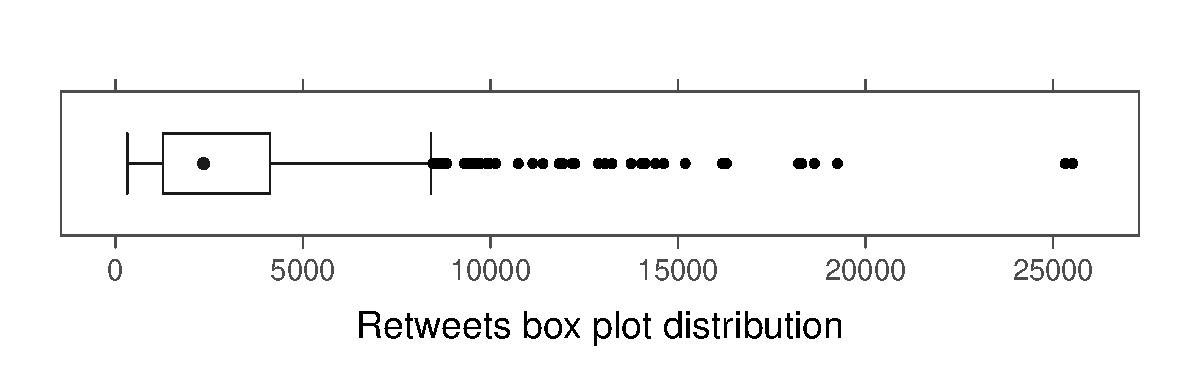
\includegraphics[width=0.89\linewidth]{figure/graphics-bw_retweets_2-1} 

}



\end{knitrout}
\end{frame}
%%%%%%%%%%%%%%%%%%%%%%%%%%%%%%%%%%%%%%%%%%%

%%%%%%%%%%%%%%%%%%%%%%%%%%%%%%%%%%%%%%%%%%%
\begin{frame}{Normal Quantile Plot}
%%%%%%%%%%%%%%%%%%%%%%%%%%%%%%%%%%%%%%%%%%%

How can I tell whether my data is sufficiently close to normal?

\begin{itemize}
\item Given data $x=(x_1, x_2, \cdots, x_n)$, compute
$$ y_{i} = \frac{x_{i} - \bar{x}}{s} $$
where $\bar{x} = mean(x)$ and $s = sd(x)$.

\item Arrange the $y$ data in increasing order: 
$$ y_{[1]} \leq y_{[2]} \leq ... \leq y_{[n]} $$

\item Find the z-scores for all the percentiles $(\frac{1}{n}, \frac{2}{n}, ..., \frac{n}{n})$ from standard normal table

\item  Plot $y_{[i]}$ values on the vertical axis against z-scores on the horizontal axis from $i = 1, ..., n$.

\end{itemize}
\end{frame}
%%%%%%%%%%%%%%%%%%%%%%%%%%%%%%%%%%%%%%%%%%%

%%%%%%%%%%%%%%%%%%%%%%%%%%%%%%%%%%%%%%%%%%%
\begin{frame}{How Normal Quantile plot looks!}
%%%%%%%%%%%%%%%%%%%%%%%%%%%%%%%%%%%%%%%%%%%

\begin{center}
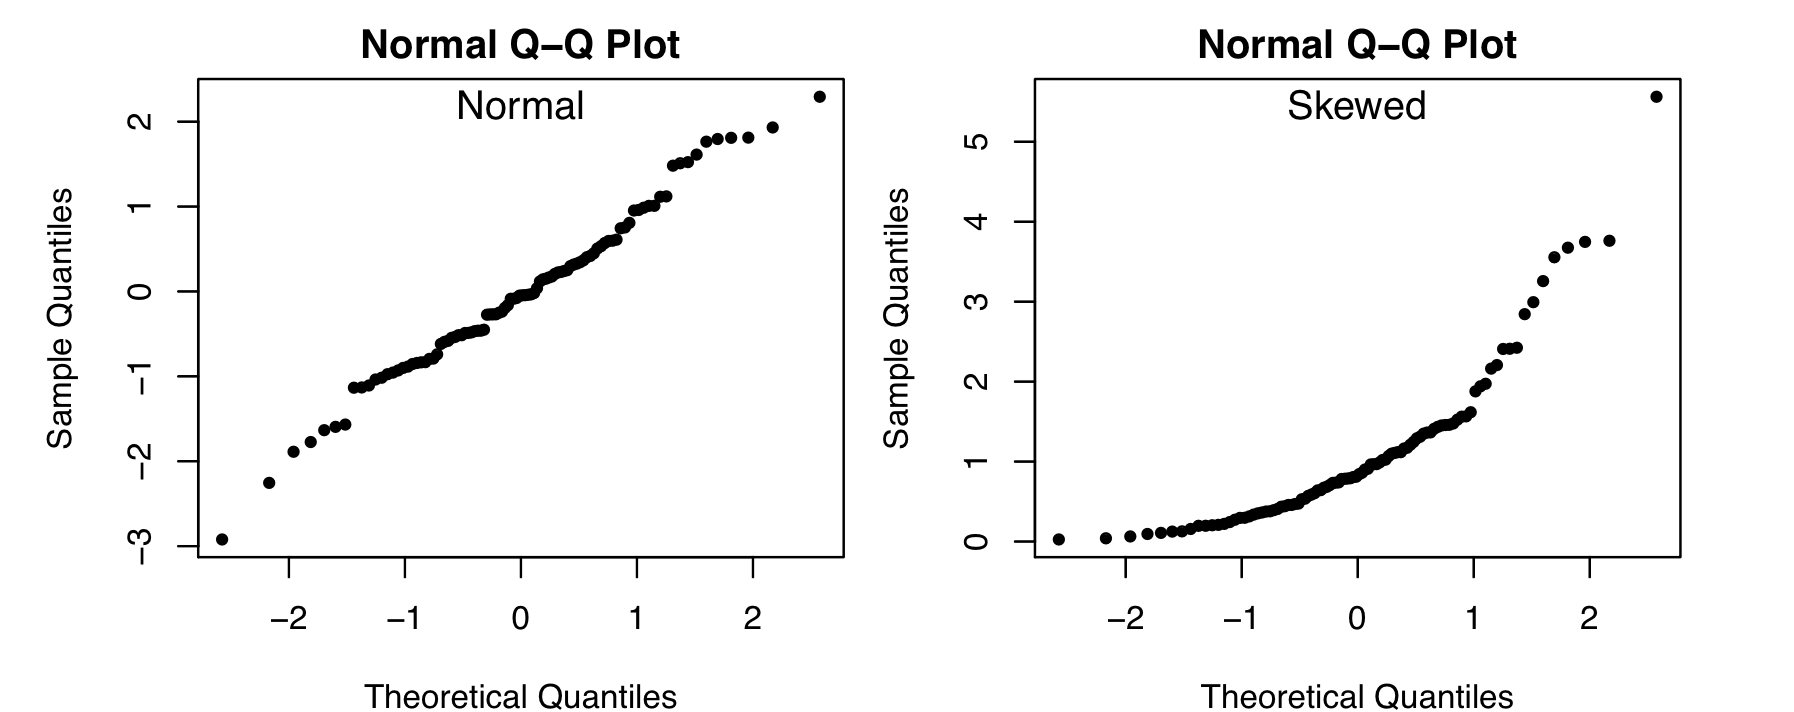
\includegraphics[height=1.5in]{P13.png}
\end{center}

If the data are approximately normal,the Q-Q plot will be \textbf{close to a straight line}.
\end{frame}
%%%%%%%%%%%%%%%%%%%%%%%%%%%%%%%%%%%%%%%%%%%

%%%%%%%%%%%%%%%%%%%%%%%%%%%%%%%%%%%%%%%%%%%
\begin{frame}{Normal Quantile Plot}
%%%%%%%%%%%%%%%%%%%%%%%%%%%%%%%%%%%%%%%%%%%

\textbf{Systematic deviations} from a straight line indicate a non-normal distribution

\begin{table}
\footnotesize
\centering
\begin{tabular}{ c  | c }			
   Heavy tails at both end & Light tails at both end \\
   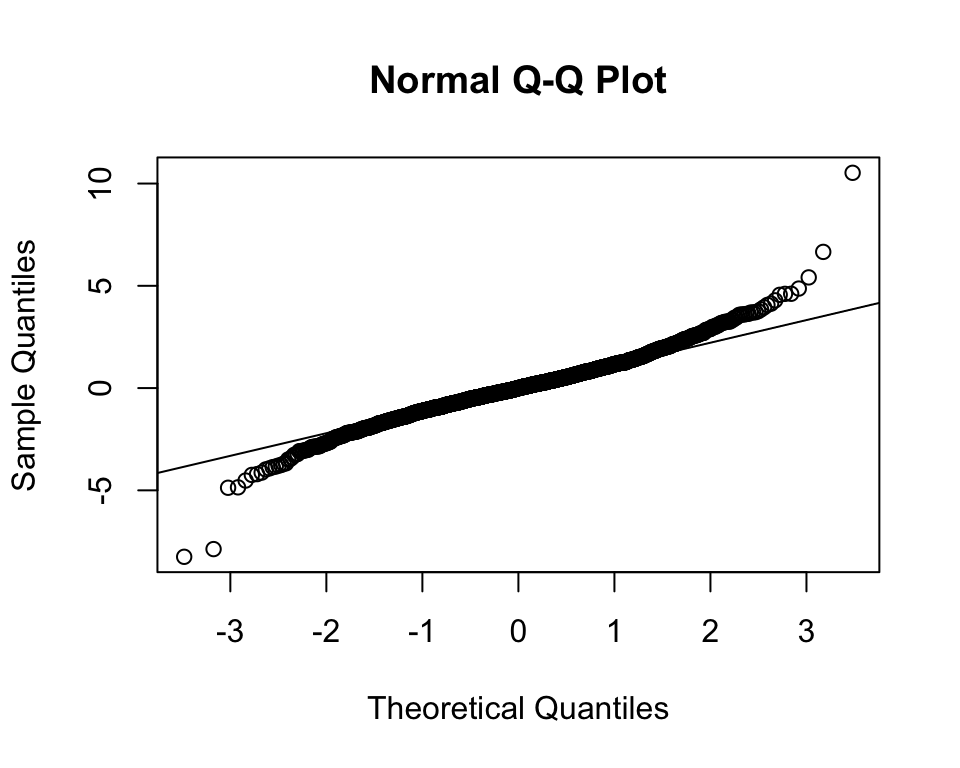
\includegraphics[height=1.1in]{QQ3.png}  &  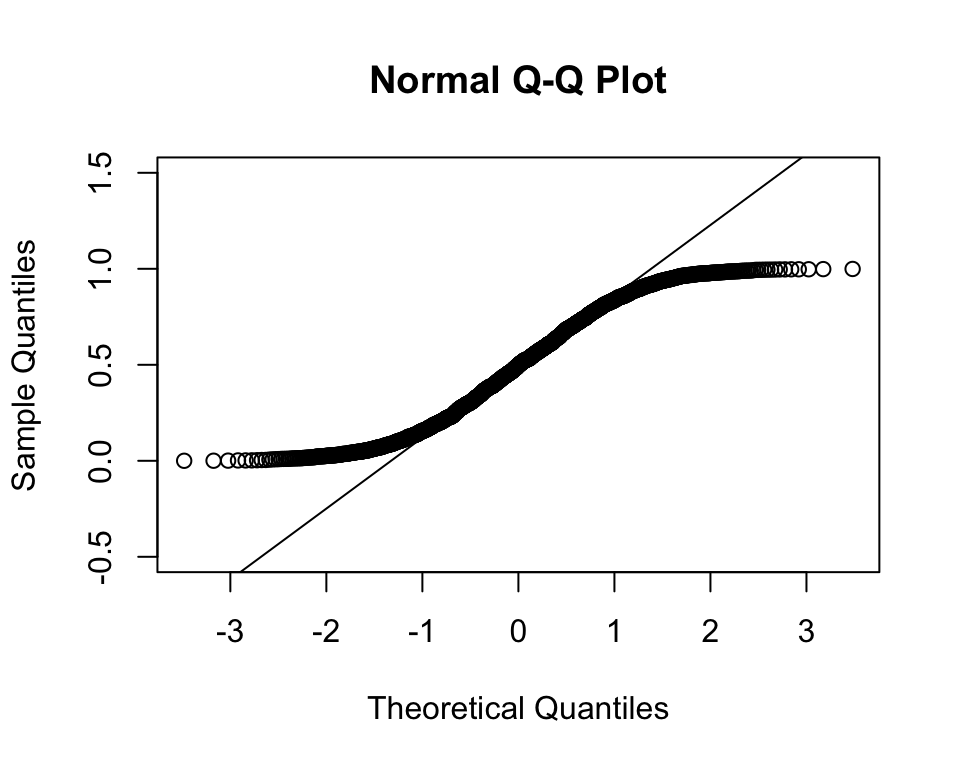
\includegraphics[height=1.1in]{QQ4.png} \\
   \hline
   Left skewed & Right skewed \\
   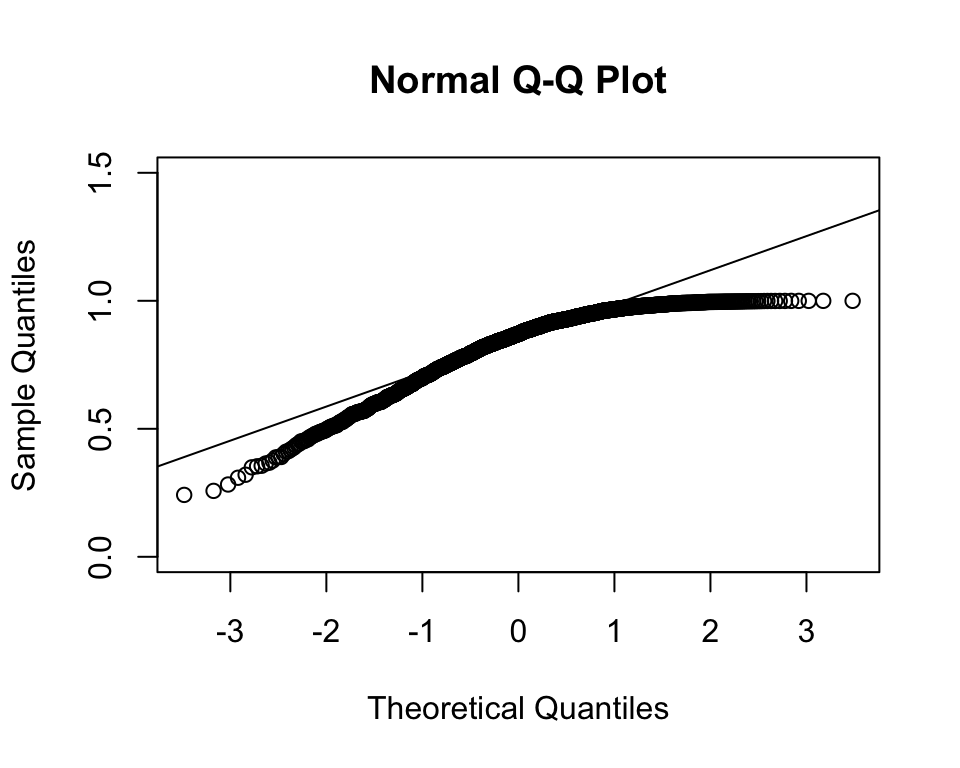
\includegraphics[height=1.1in]{QQ2.png}  &  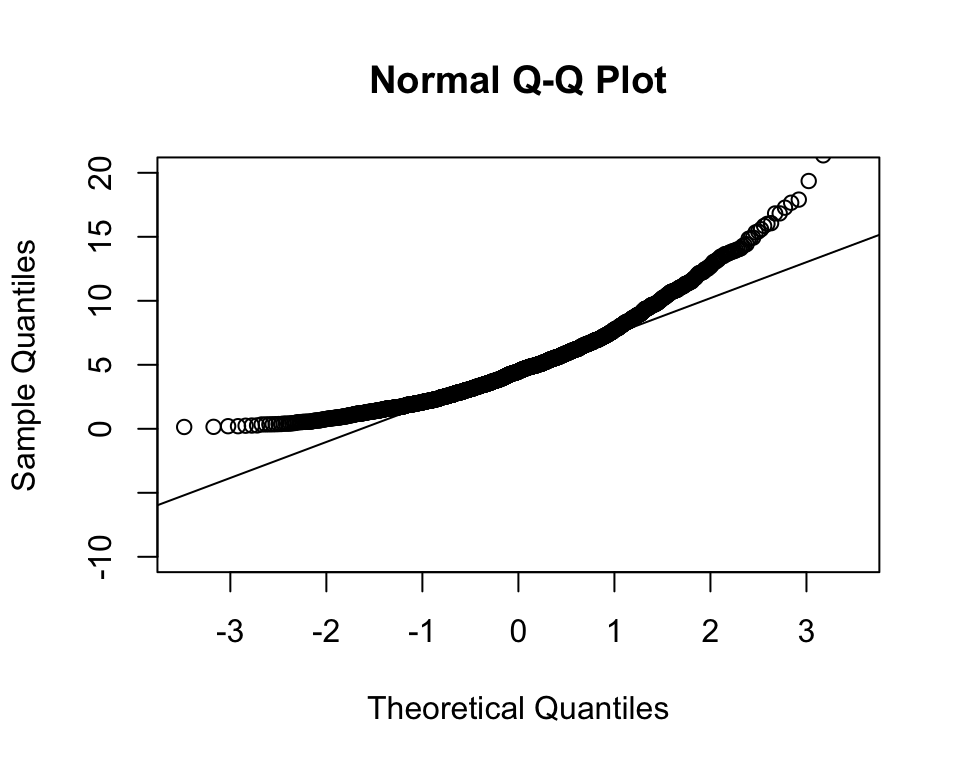
\includegraphics[height=1.1in]{QQ1.png} \\
   
\end{tabular}
\end{table}
\end{frame}
%%%%%%%%%%%%%%%%%%%%%%%%%%%%%%%%%%%%%%%%%%%

%%%%%%%%%%%%%%%%%%%%%%%%%%%%%%%%%%%%%%%%%%%
\begin{frame}{Association between Variables}
%%%%%%%%%%%%%%%%%%%%%%%%%%%%%%%%%%%%%%%%%%%

\begin{knitrout}\small
\definecolor{shadecolor}{rgb}{1, 1, 1}\color{fgcolor}

{\centering 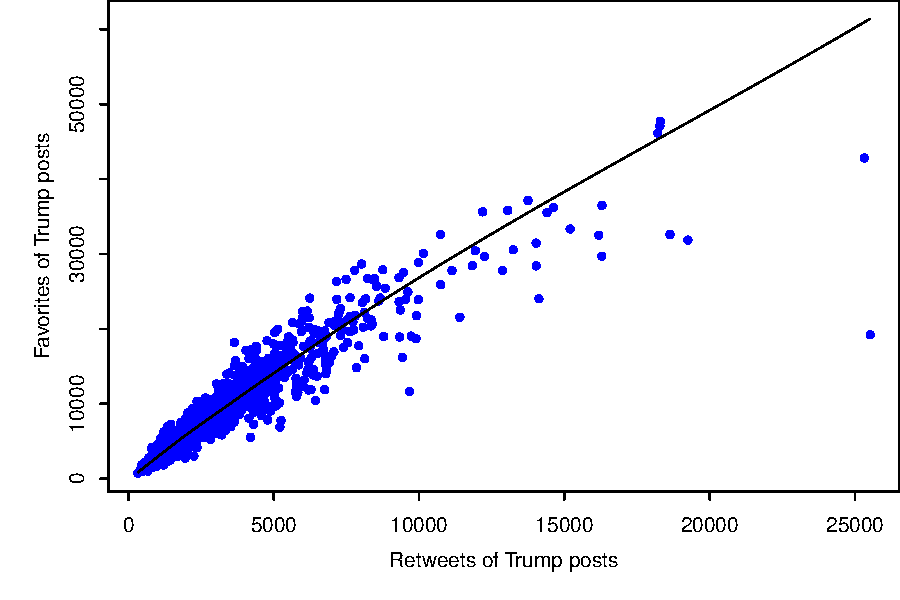
\includegraphics[width=0.99\linewidth]{figure/graphics-scatter_2-1} 

}



\end{knitrout}
\end{frame}

%%%%%%%%%%%%%%%%%%%%%%%%%%%%%%%%%%%%%%%%%%%


%%%%%%%%%%%%%%%%%%%%%%%%%%%%%%%%%%%%%%%%%%%
\begin{frame}{Describing Scatterplots}
%%%%%%%%%%%%%%%%%%%%%%%%%%%%%%%%%%%%%%%%%%%

You can describe patterns in a scatterplot in three aspects:
\begin{itemize}
\item Form: Linear, curved...
\item Direction: Positive, negative
\item Strength: Strong, weak
\end{itemize}
\end{frame}
%%%%%%%%%%%%%%%%%%%%%%%%%%%%%%%%%%%%%%%%%%%

%%%%%%%%%%%%%%%%%%%%%%%%%%%%%%%%%%%%%%%%%%%
\begin{frame}{Scatterplot}
%%%%%%%%%%%%%%%%%%%%%%%%%%%%%%%%%%%%%%%%%%%

Examples of linear relationships:
\begin{center}
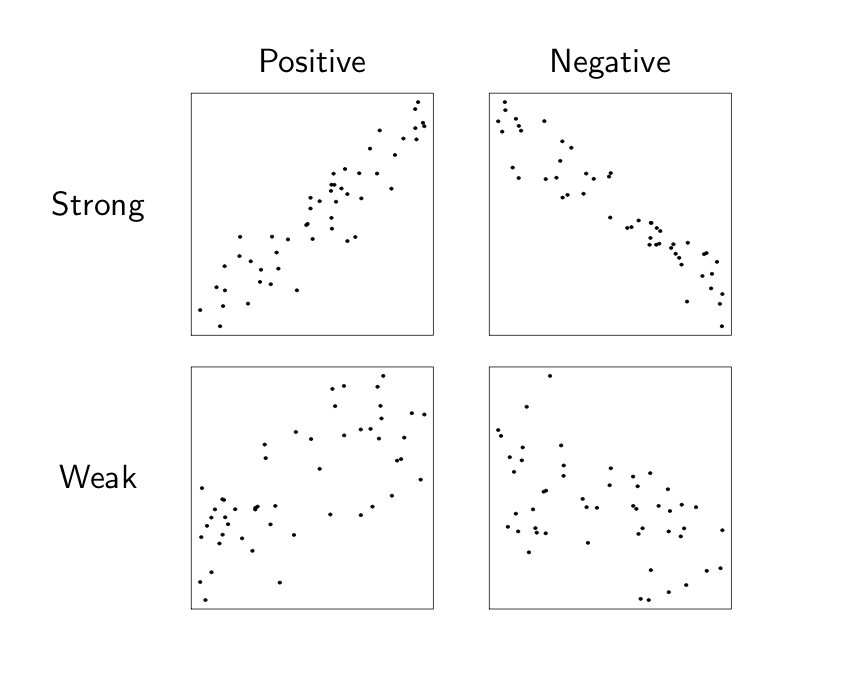
\includegraphics[height=2.5in]{P1.png}
\end{center}
\end{frame}
%%%%%%%%%%%%%%%%%%%%%%%%%%%%%%%%%%%%%%%%%%%

%%%%%%%%%%%%%%%%%%%%%%%%%%%%%%%%%%%%%%%%%%%
\begin{frame}[allowframebreaks, fragile]{Applying quantile plots to log Retweets data}
%%%%%%%%%%%%%%%%%%%%%%%%%%%%%%%%%%%%%%%%%%%

\begin{knitrout}\small
\definecolor{shadecolor}{rgb}{1, 1, 1}\color{fgcolor}\begin{kframe}
\begin{alltt}
\hlstd{mtweets} \hlkwb{<-} \hlkwd{mean}\hlstd{(}\hlkwd{log}\hlstd{(trump.data.frame}\hlopt{$}\hlstd{retweets}\hlopt{+}\hlnum{1}\hlstd{))}

\hlstd{stweets} \hlkwb{<-} \hlkwd{sd}\hlstd{(}\hlkwd{log}\hlstd{(trump.data.frame}\hlopt{$}\hlstd{retweets}\hlopt{+}\hlnum{1}\hlstd{))}

\hlstd{stdtweets} \hlkwb{=} \hlstd{(}\hlkwd{log}\hlstd{(trump.data.frame}\hlopt{$}\hlstd{retweets}\hlopt{+}\hlnum{1}\hlstd{)} \hlopt{-} \hlstd{mtweets)} \hlopt{/} \hlstd{stweets}

\hlkwd{head}\hlstd{(}\hlkwd{sort}\hlstd{(stdtweets),}\hlnum{3}\hlstd{)}
\end{alltt}
\begin{verbatim}
[1] -2.594 -2.395 -2.271
\end{verbatim}
\begin{alltt}
\hlkwd{tail}\hlstd{(}\hlkwd{sort}\hlstd{(stdtweets),}\hlnum{3}\hlstd{)}
\end{alltt}
\begin{verbatim}
[1] 2.775 3.135 3.145
\end{verbatim}
\end{kframe}
\end{knitrout}

\newpage

\begin{knitrout}\small
\definecolor{shadecolor}{rgb}{1, 1, 1}\color{fgcolor}\begin{kframe}
\begin{alltt}
\hlstd{p} \hlkwb{=} \hlkwd{c}\hlstd{(}\hlnum{0.01}\hlstd{,} \hlnum{0.025}\hlstd{,} \hlnum{0.16}\hlstd{,} \hlnum{0.25}\hlstd{,} \hlnum{0.50}\hlstd{,} \hlnum{0.75}\hlstd{,} \hlnum{0.84}\hlstd{,} \hlnum{0.975}\hlstd{,} \hlnum{0.99}\hlstd{)}
\hlstd{modelQuantile} \hlkwb{=} \hlkwd{qnorm}\hlstd{(p)}
\hlstd{modelQuantile}
\end{alltt}
\begin{verbatim}
[1] -2.3263 -1.9600 -0.9945 -0.6745  0.0000  0.6745  0.9945
[8]  1.9600  2.3263
\end{verbatim}
\begin{alltt}
\hlstd{dataQuantile} \hlkwb{=} \hlkwd{quantile}\hlstd{(stdtweets, p,} \hlkwc{na.rm}\hlstd{=}\hlnum{TRUE}\hlstd{)}
\hlstd{dataQuantile}
\end{alltt}
\begin{verbatim}
      1%     2.5%      16%      25%      50%      75% 
-1.98042 -1.77134 -1.09683 -0.79466  0.01657  0.75343 
     84%    97.5%      99% 
 1.01146  1.87581  2.36527 
\end{verbatim}
\begin{alltt}
\hlkwd{rbind}\hlstd{(dataQuantile, modelQuantile)}
\end{alltt}
\begin{verbatim}
                  1%   2.5%     16%     25%     50%    75%
dataQuantile  -1.980 -1.771 -1.0968 -0.7947 0.01657 0.7534
modelQuantile -2.326 -1.960 -0.9945 -0.6745 0.00000 0.6745
                 84% 97.5%   99%
dataQuantile  1.0115 1.876 2.365
modelQuantile 0.9945 1.960 2.326
\end{verbatim}
\end{kframe}
\end{knitrout}
\end{frame}

%%%%%%%%%%%%%%%%%%%%%%%%%%%%%%%%%%%%%%%%%%%
\begin{frame}[allowframebreaks, fragile]{Quantile plots}
%%%%%%%%%%%%%%%%%%%%%%%%%%%%%%%%%%%%%%%%%%%

\begin{knitrout}\small
\definecolor{shadecolor}{rgb}{1, 1, 1}\color{fgcolor}

{\centering 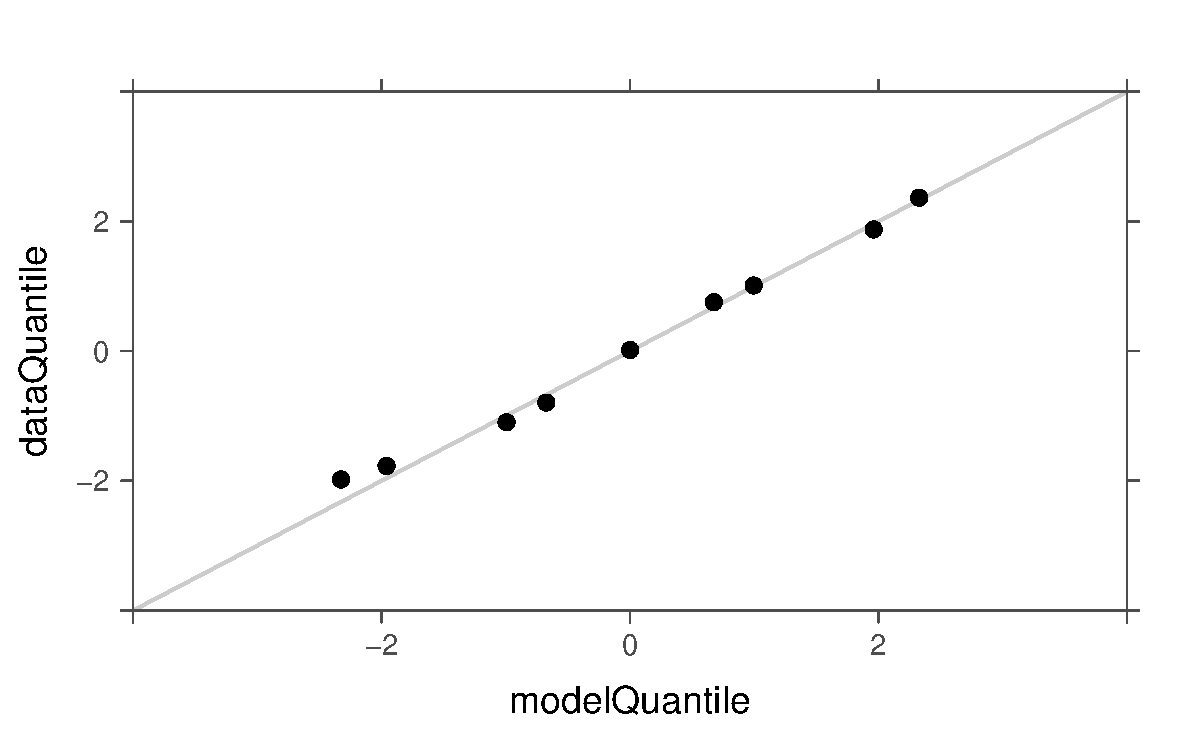
\includegraphics[width=0.89\linewidth]{figure/graphics-unnamed-chunk-23-1} 

}



\end{knitrout}
\newpage

I wish the "normal probability plot" was actually plotted like this
(much easier to read)
\begin{knitrout}\small
\definecolor{shadecolor}{rgb}{1, 1, 1}\color{fgcolor}

{\centering 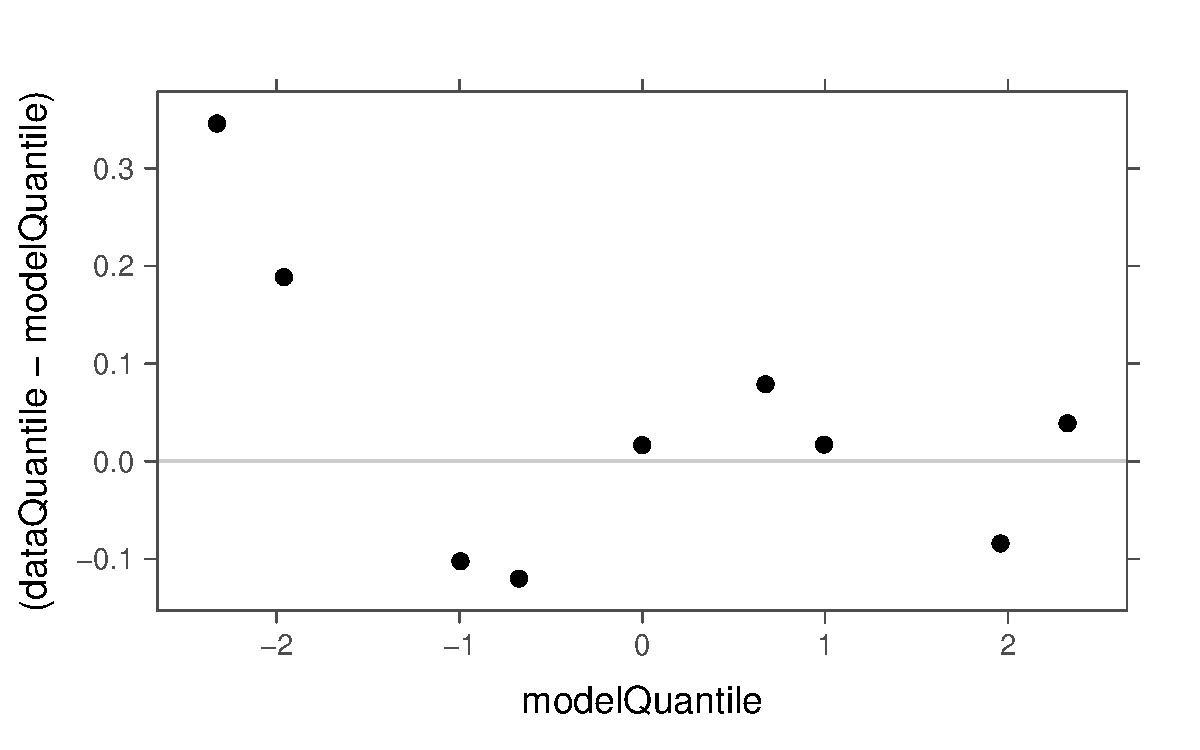
\includegraphics[width=0.89\linewidth]{figure/graphics-unnamed-chunk-24-1} 

}



\end{knitrout}
\newpage

 But here is the style of plot traditionally called the "normal probability plot" or "normal quantile plot"
\begin{knitrout}\small
\definecolor{shadecolor}{rgb}{1, 1, 1}\color{fgcolor}

{\centering 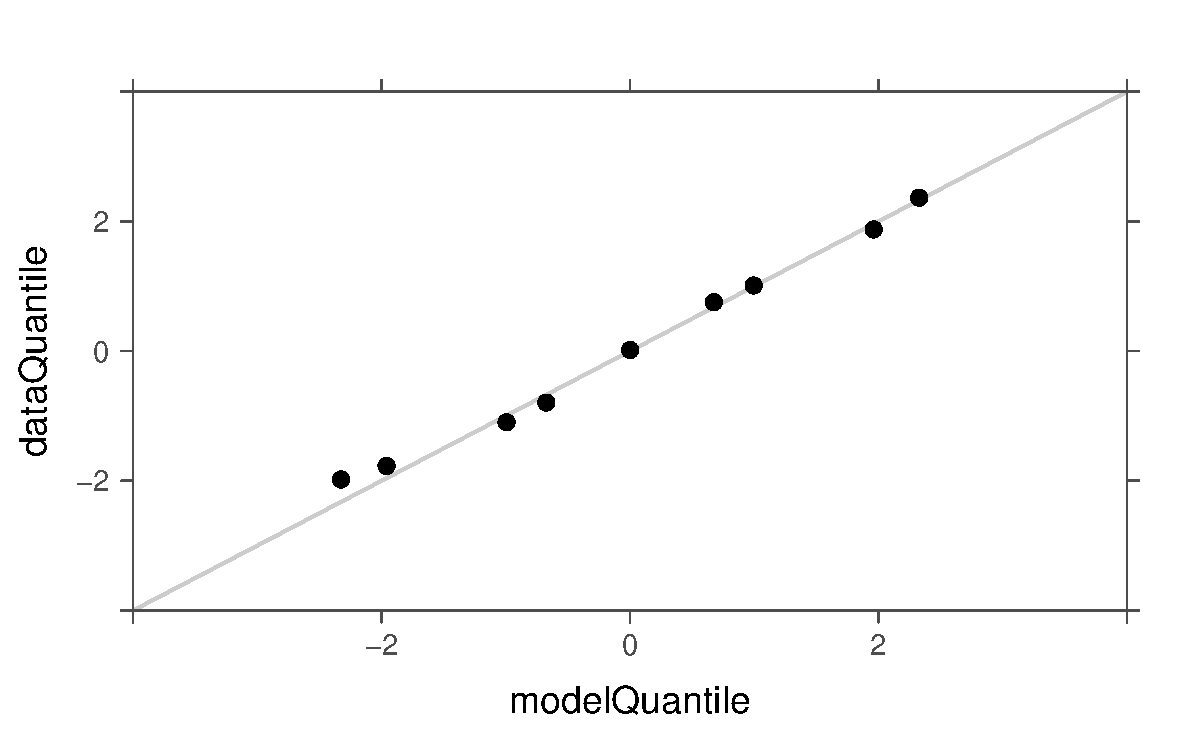
\includegraphics[width=0.89\linewidth]{figure/graphics-unnamed-chunk-25-1} 

}



\end{knitrout}

\end{frame}


%%%%%%%%%%%%%%%%%%%%%%%%%%%%%%%%%%%%%%%%%%%
\begin{frame}[allowframebreaks, fragile]{Quantile plot for Retweets Data}
%%%%%%%%%%%%%%%%%%%%%%%%%%%%%%%%%%%%%%%%%%%

\begin{knitrout}\small
\definecolor{shadecolor}{rgb}{1, 1, 1}\color{fgcolor}

{\centering 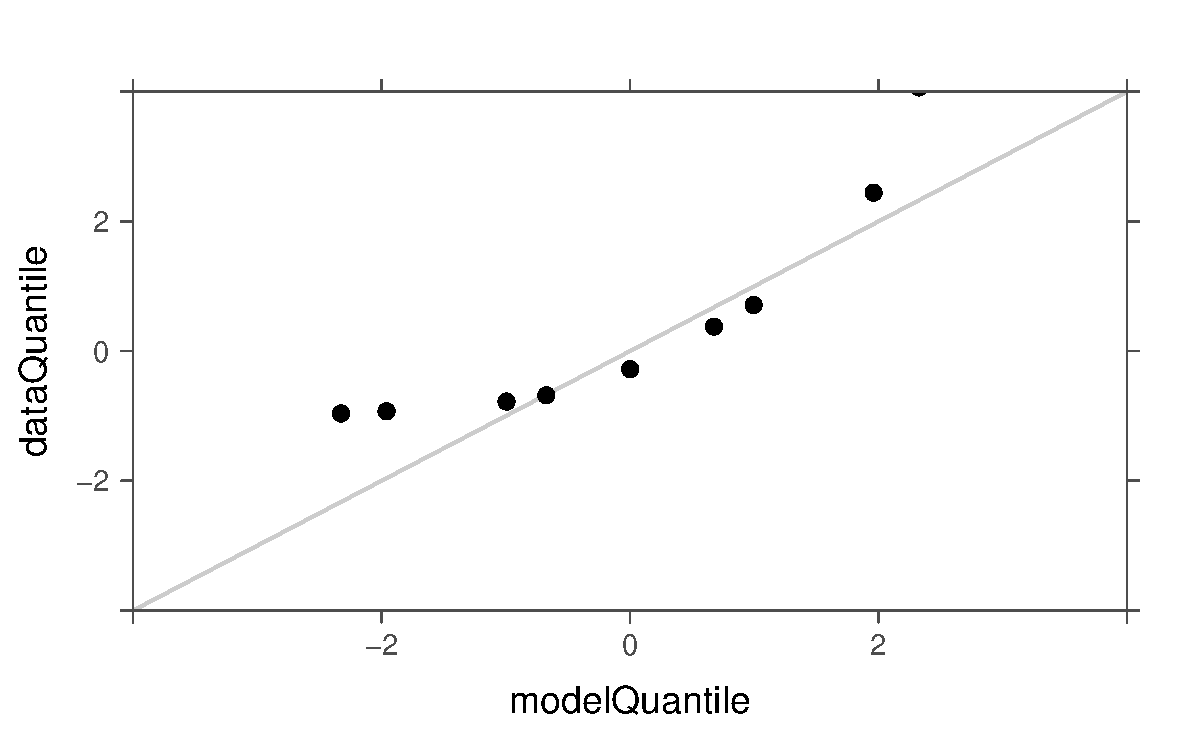
\includegraphics[width=0.89\linewidth]{figure/graphics-unnamed-chunk-26-1} 

}



\end{knitrout}
\end{frame}

%%%%%%%%%%%%%%%%%%%%%%%%%%%%%%%%%%%%%%%%%%%
\begin{frame}[allowframebreaks, fragile]
%%%%%%%%%%%%%%%%%%%%%%%%%%%%%%%%%%%%%%%%%%%

\centering \large{\textcolor{blue}{Questions?}}

\end{frame}

%%%%%%%%%%%%%% End of slides %%%%%%%%%%%%%%
%%%%%%%%%%%%%%%%%%%%%%%%%%%%%%%%%%%%%%%%%%%

\end{document}
